\documentclass[twoside]{book}

% Packages required by doxygen
\usepackage{fixltx2e}
\usepackage{calc}
\usepackage{doxygen}
\usepackage[export]{adjustbox} % also loads graphicx
\usepackage{graphicx}
\usepackage[utf8]{inputenc}
\usepackage{makeidx}
\usepackage{multicol}
\usepackage{multirow}
\PassOptionsToPackage{warn}{textcomp}
\usepackage{textcomp}
\usepackage[nointegrals]{wasysym}
\usepackage[table]{xcolor}

% Font selection
\usepackage[T1]{fontenc}
\usepackage[scaled=.90]{helvet}
\usepackage{courier}
\usepackage{amssymb}
\usepackage{sectsty}
\renewcommand{\familydefault}{\sfdefault}
\allsectionsfont{%
  \fontseries{bc}\selectfont%
  \color{darkgray}%
}
\renewcommand{\DoxyLabelFont}{%
  \fontseries{bc}\selectfont%
  \color{darkgray}%
}
\newcommand{\+}{\discretionary{\mbox{\scriptsize$\hookleftarrow$}}{}{}}

% Page & text layout
\usepackage{geometry}
\geometry{%
  a4paper,%
  top=2.5cm,%
  bottom=2.5cm,%
  left=2.5cm,%
  right=2.5cm%
}
\tolerance=750
\hfuzz=15pt
\hbadness=750
\setlength{\emergencystretch}{15pt}
\setlength{\parindent}{0cm}
\setlength{\parskip}{3ex plus 2ex minus 2ex}
\makeatletter
\renewcommand{\paragraph}{%
  \@startsection{paragraph}{4}{0ex}{-1.0ex}{1.0ex}{%
    \normalfont\normalsize\bfseries\SS@parafont%
  }%
}
\renewcommand{\subparagraph}{%
  \@startsection{subparagraph}{5}{0ex}{-1.0ex}{1.0ex}{%
    \normalfont\normalsize\bfseries\SS@subparafont%
  }%
}
\makeatother

% Headers & footers
\usepackage{fancyhdr}
\pagestyle{fancyplain}
\fancyhead[LE]{\fancyplain{}{\bfseries\thepage}}
\fancyhead[CE]{\fancyplain{}{}}
\fancyhead[RE]{\fancyplain{}{\bfseries\leftmark}}
\fancyhead[LO]{\fancyplain{}{\bfseries\rightmark}}
\fancyhead[CO]{\fancyplain{}{}}
\fancyhead[RO]{\fancyplain{}{\bfseries\thepage}}
\fancyfoot[LE]{\fancyplain{}{}}
\fancyfoot[CE]{\fancyplain{}{}}
\fancyfoot[RE]{\fancyplain{}{\bfseries\scriptsize Generated by Doxygen }}
\fancyfoot[LO]{\fancyplain{}{\bfseries\scriptsize Generated by Doxygen }}
\fancyfoot[CO]{\fancyplain{}{}}
\fancyfoot[RO]{\fancyplain{}{}}
\renewcommand{\footrulewidth}{0.4pt}
\renewcommand{\chaptermark}[1]{%
  \markboth{#1}{}%
}
\renewcommand{\sectionmark}[1]{%
  \markright{\thesection\ #1}%
}

% Indices & bibliography
\usepackage{natbib}
\usepackage[titles]{tocloft}
\setcounter{tocdepth}{3}
\setcounter{secnumdepth}{5}
\makeindex

% Hyperlinks (required, but should be loaded last)
\usepackage{ifpdf}
\ifpdf
  \usepackage[pdftex,pagebackref=true]{hyperref}
\else
  \usepackage[ps2pdf,pagebackref=true]{hyperref}
\fi
\hypersetup{%
  colorlinks=true,%
  linkcolor=blue,%
  citecolor=blue,%
  unicode%
}

% Custom commands
\newcommand{\clearemptydoublepage}{%
  \newpage{\pagestyle{empty}\cleardoublepage}%
}

\usepackage{caption}
\captionsetup{labelsep=space,justification=centering,font={bf},singlelinecheck=off,skip=4pt,position=top}

%===== C O N T E N T S =====

\begin{document}

% Titlepage & ToC
\hypersetup{pageanchor=false,
             bookmarksnumbered=true,
             pdfencoding=unicode
            }
\pagenumbering{alph}
\begin{titlepage}
\vspace*{7cm}
\begin{center}%
{\Large Bear\+Bones }\\
\vspace*{1cm}
{\large Generated by Doxygen 1.8.13}\\
\end{center}
\end{titlepage}
\clearemptydoublepage
\pagenumbering{roman}
\tableofcontents
\clearemptydoublepage
\pagenumbering{arabic}
\hypersetup{pageanchor=true}

%--- Begin generated contents ---
\chapter{Todo List}
\label{todo}
\Hypertarget{todo}

\begin{DoxyRefList}
\item[\label{todo__todo000001}%
\Hypertarget{todo__todo000001}%
Member \hyperlink{class_core_1_1_bear_bones_aae597be3992d3095612317decd91a55d}{Core\+:\+:Bear\+Bones\+:\+:Draw\+Callback} ()]Make private.  
\item[\label{todo__todo000002}%
\Hypertarget{todo__todo000002}%
Member \hyperlink{class_core_1_1_bear_bones_ad8ec7ea2b2e127f30fee7646359208e8}{Core\+:\+:Bear\+Bones\+:\+:Reshape\+Callback} (int x, int y)]Make private  
\item[\label{todo__todo000003}%
\Hypertarget{todo__todo000003}%
Member \hyperlink{class_core_1_1_bear_bones_a5d424aa025bfbefd266e7777c657ebd9}{Core\+:\+:Bear\+Bones\+:\+:Update} (int dx)]Make private.  
\item[\label{todo__todo000004}%
\Hypertarget{todo__todo000004}%
Class \hyperlink{class_objects_1_1_obj_model}{Objects\+:\+:Obj\+Model} ]Rename all vertex counts to element counts 
\end{DoxyRefList}
\chapter{Hierarchical Index}
\section{Class Hierarchy}
This inheritance list is sorted roughly, but not completely, alphabetically\+:\begin{DoxyCompactList}
\item \contentsline{section}{Collision\+:\+:A\+A\+BB}{\pageref{class_collision_1_1_a_a_b_b}}{}
\item \contentsline{section}{Core\+:\+:Bear\+Bones}{\pageref{class_core_1_1_bear_bones}}{}
\item \contentsline{section}{Objects\+:\+:Camera}{\pageref{class_objects_1_1_camera}}{}
\item \contentsline{section}{Objects\+:\+:Entity}{\pageref{class_objects_1_1_entity}}{}
\begin{DoxyCompactList}
\item \contentsline{section}{Objects\+:\+:Static\+Entity}{\pageref{class_objects_1_1_static_entity}}{}
\end{DoxyCompactList}
\item \contentsline{section}{Input\+:\+:Input\+Manager}{\pageref{class_input_1_1_input_manager}}{}
\item \contentsline{section}{Util\+:\+:Math\+Util}{\pageref{class_util_1_1_math_util}}{}
\item \contentsline{section}{Collision\+:\+:O\+BB}{\pageref{class_collision_1_1_o_b_b}}{}
\item \contentsline{section}{Objects\+:\+:Obj\+Model}{\pageref{class_objects_1_1_obj_model}}{}
\item \contentsline{section}{Rendering\+:\+:Renderer}{\pageref{class_rendering_1_1_renderer}}{}
\item \contentsline{section}{Objects\+:\+:Resource\+Loader}{\pageref{class_objects_1_1_resource_loader}}{}
\item \contentsline{section}{Shaders\+:\+:Shader\+Base}{\pageref{class_shaders_1_1_shader_base}}{}
\begin{DoxyCompactList}
\item \contentsline{section}{Shaders\+:\+:Static\+Shader}{\pageref{class_shaders_1_1_static_shader}}{}
\end{DoxyCompactList}
\item \contentsline{section}{Objects\+:\+:Texture}{\pageref{class_objects_1_1_texture}}{}
\item \contentsline{section}{Objects\+:\+:World}{\pageref{class_objects_1_1_world}}{}
\end{DoxyCompactList}

\chapter{Class Index}
\section{Class List}
Here are the classes, structs, unions and interfaces with brief descriptions\+:\begin{DoxyCompactList}
\item\contentsline{section}{\hyperlink{class_collision_1_1_a_a_b_b}{Collision\+::\+A\+A\+BB} }{\pageref{class_collision_1_1_a_a_b_b}}{}
\item\contentsline{section}{\hyperlink{class_core_1_1_bear_bones}{Core\+::\+Bear\+Bones} }{\pageref{class_core_1_1_bear_bones}}{}
\item\contentsline{section}{\hyperlink{class_objects_1_1_camera}{Objects\+::\+Camera} }{\pageref{class_objects_1_1_camera}}{}
\item\contentsline{section}{\hyperlink{class_objects_1_1_entity}{Objects\+::\+Entity} }{\pageref{class_objects_1_1_entity}}{}
\item\contentsline{section}{\hyperlink{class_input_1_1_input_manager}{Input\+::\+Input\+Manager} }{\pageref{class_input_1_1_input_manager}}{}
\item\contentsline{section}{\hyperlink{class_util_1_1_math_util}{Util\+::\+Math\+Util} }{\pageref{class_util_1_1_math_util}}{}
\item\contentsline{section}{\hyperlink{class_collision_1_1_o_b_b}{Collision\+::\+O\+BB} }{\pageref{class_collision_1_1_o_b_b}}{}
\item\contentsline{section}{\hyperlink{class_objects_1_1_obj_model}{Objects\+::\+Obj\+Model} }{\pageref{class_objects_1_1_obj_model}}{}
\item\contentsline{section}{\hyperlink{class_rendering_1_1_renderer}{Rendering\+::\+Renderer} }{\pageref{class_rendering_1_1_renderer}}{}
\item\contentsline{section}{\hyperlink{class_objects_1_1_resource_loader}{Objects\+::\+Resource\+Loader} }{\pageref{class_objects_1_1_resource_loader}}{}
\item\contentsline{section}{\hyperlink{class_shaders_1_1_shader_base}{Shaders\+::\+Shader\+Base} }{\pageref{class_shaders_1_1_shader_base}}{}
\item\contentsline{section}{\hyperlink{class_objects_1_1_static_entity}{Objects\+::\+Static\+Entity} }{\pageref{class_objects_1_1_static_entity}}{}
\item\contentsline{section}{\hyperlink{class_shaders_1_1_static_shader}{Shaders\+::\+Static\+Shader} }{\pageref{class_shaders_1_1_static_shader}}{}
\item\contentsline{section}{\hyperlink{class_objects_1_1_texture}{Objects\+::\+Texture} }{\pageref{class_objects_1_1_texture}}{}
\item\contentsline{section}{\hyperlink{class_objects_1_1_world}{Objects\+::\+World} }{\pageref{class_objects_1_1_world}}{}
\end{DoxyCompactList}

\chapter{Class Documentation}
\hypertarget{class_collision_1_1_a_a_b_b}{}\section{Collision\+:\+:A\+A\+BB Class Reference}
\label{class_collision_1_1_a_a_b_b}\index{Collision\+::\+A\+A\+BB@{Collision\+::\+A\+A\+BB}}


{\ttfamily \#include $<$A\+A\+B\+B.\+h$>$}

\subsection*{Public Member Functions}
\begin{DoxyCompactItemize}
\item 
\mbox{\Hypertarget{class_collision_1_1_a_a_b_b_aa68eab372bdbba7e4752d42fa4166d1f}\label{class_collision_1_1_a_a_b_b_aa68eab372bdbba7e4752d42fa4166d1f}} 
{\bfseries A\+A\+BB} (const \hyperlink{class_collision_1_1_a_a_b_b}{A\+A\+BB} \&other)
\item 
void \hyperlink{class_collision_1_1_a_a_b_b_a863ba998549280e4eada0916abc7c958}{Set\+Min\+Bounds} (glm\+::vec3 min\+Bounds)
\item 
void \hyperlink{class_collision_1_1_a_a_b_b_a4ef21c9f5d611f52c946b0b3c92712e2}{Set\+Min\+Bounds} (float x, float y, float z)
\item 
void \hyperlink{class_collision_1_1_a_a_b_b_a5fae8760f90ffd4f7bf6ce5f0903d7a0}{Set\+Max\+Bounds} (glm\+::vec3 max\+Bounds)
\item 
void \hyperlink{class_collision_1_1_a_a_b_b_a6ce73a9cb95d8d5d8ab19c625be032cd}{Set\+Max\+Bounds} (float x, float y, float z)
\item 
glm\+::vec3 \hyperlink{class_collision_1_1_a_a_b_b_a4fb67a336a9dccc1e5df1742e5215a82}{Get\+Min\+Bounds} ()
\item 
glm\+::vec3 \hyperlink{class_collision_1_1_a_a_b_b_a63411027d9f8b4300657afdeaa11f477}{Get\+Max\+Bounds} ()
\end{DoxyCompactItemize}


\subsection{Detailed Description}
An Axis Aligned Bounding Box. \begin{DoxyAuthor}{Author}
Mathew Causby 
\end{DoxyAuthor}
\begin{DoxyVersion}{Version}
0.\+1 
\end{DoxyVersion}


Definition at line 12 of file A\+A\+B\+B.\+h.



\subsection{Member Function Documentation}
\mbox{\Hypertarget{class_collision_1_1_a_a_b_b_a63411027d9f8b4300657afdeaa11f477}\label{class_collision_1_1_a_a_b_b_a63411027d9f8b4300657afdeaa11f477}} 
\index{Collision\+::\+A\+A\+BB@{Collision\+::\+A\+A\+BB}!Get\+Max\+Bounds@{Get\+Max\+Bounds}}
\index{Get\+Max\+Bounds@{Get\+Max\+Bounds}!Collision\+::\+A\+A\+BB@{Collision\+::\+A\+A\+BB}}
\subsubsection{\texorpdfstring{Get\+Max\+Bounds()}{GetMaxBounds()}}
{\footnotesize\ttfamily glm\+::vec3 Collision\+::\+A\+A\+B\+B\+::\+Get\+Max\+Bounds (\begin{DoxyParamCaption}{ }\end{DoxyParamCaption})}

Gets the maximum bounds of the \hyperlink{class_collision_1_1_a_a_b_b}{A\+A\+BB} \begin{DoxyReturn}{Returns}
The maximum bounds 
\end{DoxyReturn}


Definition at line 49 of file A\+A\+B\+B.\+cpp.

\mbox{\Hypertarget{class_collision_1_1_a_a_b_b_a4fb67a336a9dccc1e5df1742e5215a82}\label{class_collision_1_1_a_a_b_b_a4fb67a336a9dccc1e5df1742e5215a82}} 
\index{Collision\+::\+A\+A\+BB@{Collision\+::\+A\+A\+BB}!Get\+Min\+Bounds@{Get\+Min\+Bounds}}
\index{Get\+Min\+Bounds@{Get\+Min\+Bounds}!Collision\+::\+A\+A\+BB@{Collision\+::\+A\+A\+BB}}
\subsubsection{\texorpdfstring{Get\+Min\+Bounds()}{GetMinBounds()}}
{\footnotesize\ttfamily glm\+::vec3 Collision\+::\+A\+A\+B\+B\+::\+Get\+Min\+Bounds (\begin{DoxyParamCaption}{ }\end{DoxyParamCaption})}

Gets the minimum bounds of the \hyperlink{class_collision_1_1_a_a_b_b}{A\+A\+BB} \begin{DoxyReturn}{Returns}
The minimum bounds 
\end{DoxyReturn}


Definition at line 44 of file A\+A\+B\+B.\+cpp.

\mbox{\Hypertarget{class_collision_1_1_a_a_b_b_a5fae8760f90ffd4f7bf6ce5f0903d7a0}\label{class_collision_1_1_a_a_b_b_a5fae8760f90ffd4f7bf6ce5f0903d7a0}} 
\index{Collision\+::\+A\+A\+BB@{Collision\+::\+A\+A\+BB}!Set\+Max\+Bounds@{Set\+Max\+Bounds}}
\index{Set\+Max\+Bounds@{Set\+Max\+Bounds}!Collision\+::\+A\+A\+BB@{Collision\+::\+A\+A\+BB}}
\subsubsection{\texorpdfstring{Set\+Max\+Bounds()}{SetMaxBounds()}\hspace{0.1cm}{\footnotesize\ttfamily [1/2]}}
{\footnotesize\ttfamily void Collision\+::\+A\+A\+B\+B\+::\+Set\+Max\+Bounds (\begin{DoxyParamCaption}\item[{glm\+::vec3}]{max\+Bounds }\end{DoxyParamCaption})}

Sets the maximum bounds of the \hyperlink{class_collision_1_1_a_a_b_b}{A\+A\+BB} 
\begin{DoxyParams}[1]{Parameters}
\mbox{\tt in}  & {\em max\+Bounds} & The maximum bounds \\
\hline
\end{DoxyParams}


Definition at line 32 of file A\+A\+B\+B.\+cpp.

\mbox{\Hypertarget{class_collision_1_1_a_a_b_b_a6ce73a9cb95d8d5d8ab19c625be032cd}\label{class_collision_1_1_a_a_b_b_a6ce73a9cb95d8d5d8ab19c625be032cd}} 
\index{Collision\+::\+A\+A\+BB@{Collision\+::\+A\+A\+BB}!Set\+Max\+Bounds@{Set\+Max\+Bounds}}
\index{Set\+Max\+Bounds@{Set\+Max\+Bounds}!Collision\+::\+A\+A\+BB@{Collision\+::\+A\+A\+BB}}
\subsubsection{\texorpdfstring{Set\+Max\+Bounds()}{SetMaxBounds()}\hspace{0.1cm}{\footnotesize\ttfamily [2/2]}}
{\footnotesize\ttfamily void Collision\+::\+A\+A\+B\+B\+::\+Set\+Max\+Bounds (\begin{DoxyParamCaption}\item[{float}]{x,  }\item[{float}]{y,  }\item[{float}]{z }\end{DoxyParamCaption})}

Sets the maximum bounds of the \hyperlink{class_collision_1_1_a_a_b_b}{A\+A\+BB} 
\begin{DoxyParams}[1]{Parameters}
\mbox{\tt in}  & {\em x} & The X value \\
\hline
\mbox{\tt in}  & {\em y} & T\+He Y value \\
\hline
\mbox{\tt in}  & {\em z} & The Z value \\
\hline
\end{DoxyParams}


Definition at line 37 of file A\+A\+B\+B.\+cpp.

\mbox{\Hypertarget{class_collision_1_1_a_a_b_b_a863ba998549280e4eada0916abc7c958}\label{class_collision_1_1_a_a_b_b_a863ba998549280e4eada0916abc7c958}} 
\index{Collision\+::\+A\+A\+BB@{Collision\+::\+A\+A\+BB}!Set\+Min\+Bounds@{Set\+Min\+Bounds}}
\index{Set\+Min\+Bounds@{Set\+Min\+Bounds}!Collision\+::\+A\+A\+BB@{Collision\+::\+A\+A\+BB}}
\subsubsection{\texorpdfstring{Set\+Min\+Bounds()}{SetMinBounds()}\hspace{0.1cm}{\footnotesize\ttfamily [1/2]}}
{\footnotesize\ttfamily void Collision\+::\+A\+A\+B\+B\+::\+Set\+Min\+Bounds (\begin{DoxyParamCaption}\item[{glm\+::vec3}]{min\+Bounds }\end{DoxyParamCaption})}

Sets the minimum bounds of the \hyperlink{class_collision_1_1_a_a_b_b}{A\+A\+BB} 
\begin{DoxyParams}[1]{Parameters}
\mbox{\tt in}  & {\em min\+Bounds} & The minimum bounds. \\
\hline
\end{DoxyParams}


Definition at line 20 of file A\+A\+B\+B.\+cpp.

\mbox{\Hypertarget{class_collision_1_1_a_a_b_b_a4ef21c9f5d611f52c946b0b3c92712e2}\label{class_collision_1_1_a_a_b_b_a4ef21c9f5d611f52c946b0b3c92712e2}} 
\index{Collision\+::\+A\+A\+BB@{Collision\+::\+A\+A\+BB}!Set\+Min\+Bounds@{Set\+Min\+Bounds}}
\index{Set\+Min\+Bounds@{Set\+Min\+Bounds}!Collision\+::\+A\+A\+BB@{Collision\+::\+A\+A\+BB}}
\subsubsection{\texorpdfstring{Set\+Min\+Bounds()}{SetMinBounds()}\hspace{0.1cm}{\footnotesize\ttfamily [2/2]}}
{\footnotesize\ttfamily void Collision\+::\+A\+A\+B\+B\+::\+Set\+Min\+Bounds (\begin{DoxyParamCaption}\item[{float}]{x,  }\item[{float}]{y,  }\item[{float}]{z }\end{DoxyParamCaption})}

Sets the minimum bounds of the \hyperlink{class_collision_1_1_a_a_b_b}{A\+A\+BB} 
\begin{DoxyParams}[1]{Parameters}
\mbox{\tt in}  & {\em x} & The X value \\
\hline
\mbox{\tt in}  & {\em y} & T\+He Y value \\
\hline
\mbox{\tt in}  & {\em z} & The Z value \\
\hline
\end{DoxyParams}


Definition at line 25 of file A\+A\+B\+B.\+cpp.



The documentation for this class was generated from the following files\+:\begin{DoxyCompactItemize}
\item 
Bear\+Bones-\/master/\+Bear\+Bones/src/\+Collision/A\+A\+B\+B.\+h\item 
Bear\+Bones-\/master/\+Bear\+Bones/src/\+Collision/A\+A\+B\+B.\+cpp\end{DoxyCompactItemize}

\hypertarget{class_core_1_1_bear_bones}{}\section{Core\+:\+:Bear\+Bones Class Reference}
\label{class_core_1_1_bear_bones}\index{Core\+::\+Bear\+Bones@{Core\+::\+Bear\+Bones}}


{\ttfamily \#include $<$Bear\+Bones.\+h$>$}

\subsection*{Public Member Functions}
\begin{DoxyCompactItemize}
\item 
int \hyperlink{class_core_1_1_bear_bones_a4023165c84d690ba6bade029bc60a710}{Initialize\+Window} (int $\ast$argc, char $\ast$$\ast$argv, int winX, int winY)
\item 
void \hyperlink{class_core_1_1_bear_bones_ad4258f21b446ccdc93f711bae6aae813}{Begin\+Main\+Game\+Loop} ()
\item 
void \hyperlink{class_core_1_1_bear_bones_aae597be3992d3095612317decd91a55d}{Draw\+Callback} ()
\item 
void \hyperlink{class_core_1_1_bear_bones_ad8ec7ea2b2e127f30fee7646359208e8}{Reshape\+Callback} (int x, int y)
\item 
void \hyperlink{class_core_1_1_bear_bones_a5d424aa025bfbefd266e7777c657ebd9}{Update} (int dx)
\item 
void \hyperlink{class_core_1_1_bear_bones_a369f24d6903dc2cfb5c766fbbfdcdfb8}{Get\+Window\+Size} (int \&x, int \&y)
\item 
void \hyperlink{class_core_1_1_bear_bones_a3e5b6f1994fdf8db744aba2f5a7547be}{Quit} ()
\item 
void \hyperlink{class_core_1_1_bear_bones_a980bca579db7dfbaebe2e8636660d0e2}{Set\+Update\+Callback} (f callback)
\item 
void \hyperlink{class_core_1_1_bear_bones_adf0f0c14fc729a3c7ac51297430b824d}{Get\+Resource\+Loader} (std\+::shared\+\_\+ptr$<$ \hyperlink{class_objects_1_1_resource_loader}{Objects\+::\+Resource\+Loader} $>$ \&loader)
\item 
void \hyperlink{class_core_1_1_bear_bones_af5f9add95ce3557aa9f045c55a61a760}{Get\+World} (std\+::shared\+\_\+ptr$<$ \hyperlink{class_objects_1_1_world}{Objects\+::\+World} $>$ \&world)
\item 
void \hyperlink{class_core_1_1_bear_bones_a4566808b082431ab19831dee7afd700b}{Get\+Camera} (std\+::shared\+\_\+ptr$<$ \hyperlink{class_objects_1_1_camera}{Objects\+::\+Camera} $>$ \&camera)
\end{DoxyCompactItemize}
\subsection*{Static Public Member Functions}
\begin{DoxyCompactItemize}
\item 
static \hyperlink{class_core_1_1_bear_bones}{Bear\+Bones} $\ast$ \hyperlink{class_core_1_1_bear_bones_acd30744bc23c254b1c211b3370c5285b}{Get\+Instance} ()
\item 
\mbox{\Hypertarget{class_core_1_1_bear_bones_a5a1ebfac1f03eb109d16f6eb5323aa7b}\label{class_core_1_1_bear_bones_a5a1ebfac1f03eb109d16f6eb5323aa7b}} 
static void {\bfseries Static\+Draw\+Callback} ()
\item 
\mbox{\Hypertarget{class_core_1_1_bear_bones_a9f614a631570c27302b547f8e455b490}\label{class_core_1_1_bear_bones_a9f614a631570c27302b547f8e455b490}} 
static void {\bfseries Static\+Reshape\+Callback} (int x, int y)
\item 
\mbox{\Hypertarget{class_core_1_1_bear_bones_a2f3124566f319322c8ed018ef26d70cf}\label{class_core_1_1_bear_bones_a2f3124566f319322c8ed018ef26d70cf}} 
static void {\bfseries Static\+Keyboard\+Callback} (unsigned char key, int x, int y)
\item 
\mbox{\Hypertarget{class_core_1_1_bear_bones_ada1a138721b6c52340048737a7da47ff}\label{class_core_1_1_bear_bones_ada1a138721b6c52340048737a7da47ff}} 
static void {\bfseries Static\+Keyboard\+Up\+Callback} (unsigned char key, int x, int y)
\item 
\mbox{\Hypertarget{class_core_1_1_bear_bones_a57181e3fdb45a9a76a52c0880e097aff}\label{class_core_1_1_bear_bones_a57181e3fdb45a9a76a52c0880e097aff}} 
static void {\bfseries Static\+Special\+Keyboard\+Callback} (int key, int x, int y)
\item 
\mbox{\Hypertarget{class_core_1_1_bear_bones_a024876e1246d99395cecc70c7217a4a5}\label{class_core_1_1_bear_bones_a024876e1246d99395cecc70c7217a4a5}} 
static void {\bfseries Static\+Special\+Keyboard\+Up\+Callback} (int key, int x, int y)
\item 
\mbox{\Hypertarget{class_core_1_1_bear_bones_a434c29a5fc3f34cf83f81403ea9699c7}\label{class_core_1_1_bear_bones_a434c29a5fc3f34cf83f81403ea9699c7}} 
static void {\bfseries Static\+Mouse\+Callback} (int button, int state, int x, int y)
\item 
\mbox{\Hypertarget{class_core_1_1_bear_bones_a1881e977aae064d71ef78ad8cdef6df8}\label{class_core_1_1_bear_bones_a1881e977aae064d71ef78ad8cdef6df8}} 
static void {\bfseries Static\+Mouse\+Position\+Callback} (int x, int y)
\item 
\mbox{\Hypertarget{class_core_1_1_bear_bones_a5e45a19a314a961e81ab5651f4fbee19}\label{class_core_1_1_bear_bones_a5e45a19a314a961e81ab5651f4fbee19}} 
static void {\bfseries Static\+Update\+Callback} (int value)
\item 
\mbox{\Hypertarget{class_core_1_1_bear_bones_ae6a4688406df0c1b652a1a0e6c82a923}\label{class_core_1_1_bear_bones_ae6a4688406df0c1b652a1a0e6c82a923}} 
static void A\+P\+I\+E\+N\+T\+RY {\bfseries Static\+Message\+Callback} (G\+Lenum source, G\+Lenum type, G\+Luint id, G\+Lenum severity, G\+Lsizei length, const G\+Lchar $\ast$message, const void $\ast$user\+Param)
\end{DoxyCompactItemize}


\subsection{Detailed Description}
This is the main class of the engine. It is a singleton class that manages all of the engine\textquotesingle{}s resources, and controls the interfaces with Free\+G\+L\+UT. \begin{DoxyAuthor}{Author}
Mathew Causby 
\end{DoxyAuthor}
\begin{DoxyVersion}{Version}
0.\+1 
\end{DoxyVersion}


Definition at line 24 of file Bear\+Bones.\+h.



\subsection{Member Function Documentation}
\mbox{\Hypertarget{class_core_1_1_bear_bones_ad4258f21b446ccdc93f711bae6aae813}\label{class_core_1_1_bear_bones_ad4258f21b446ccdc93f711bae6aae813}} 
\index{Core\+::\+Bear\+Bones@{Core\+::\+Bear\+Bones}!Begin\+Main\+Game\+Loop@{Begin\+Main\+Game\+Loop}}
\index{Begin\+Main\+Game\+Loop@{Begin\+Main\+Game\+Loop}!Core\+::\+Bear\+Bones@{Core\+::\+Bear\+Bones}}
\subsubsection{\texorpdfstring{Begin\+Main\+Game\+Loop()}{BeginMainGameLoop()}}
{\footnotesize\ttfamily void Core\+::\+Bear\+Bones\+::\+Begin\+Main\+Game\+Loop (\begin{DoxyParamCaption}{ }\end{DoxyParamCaption})}

Begins the main game loop. Will keep calling the update callback. 

Definition at line 75 of file Bear\+Bones.\+cpp.

\mbox{\Hypertarget{class_core_1_1_bear_bones_aae597be3992d3095612317decd91a55d}\label{class_core_1_1_bear_bones_aae597be3992d3095612317decd91a55d}} 
\index{Core\+::\+Bear\+Bones@{Core\+::\+Bear\+Bones}!Draw\+Callback@{Draw\+Callback}}
\index{Draw\+Callback@{Draw\+Callback}!Core\+::\+Bear\+Bones@{Core\+::\+Bear\+Bones}}
\subsubsection{\texorpdfstring{Draw\+Callback()}{DrawCallback()}}
{\footnotesize\ttfamily void Core\+::\+Bear\+Bones\+::\+Draw\+Callback (\begin{DoxyParamCaption}{ }\end{DoxyParamCaption})}

The draw callback, called internally. \begin{DoxyRefDesc}{Todo}
\item[\hyperlink{todo__todo000001}{Todo}]Make private. \end{DoxyRefDesc}


Definition at line 81 of file Bear\+Bones.\+cpp.

Here is the caller graph for this function\+:
\nopagebreak
\begin{figure}[H]
\begin{center}
\leavevmode
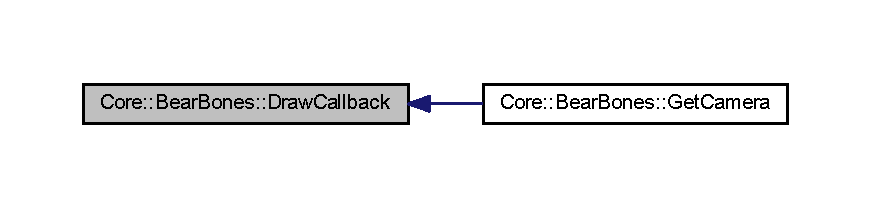
\includegraphics[width=350pt]{class_core_1_1_bear_bones_aae597be3992d3095612317decd91a55d_icgraph}
\end{center}
\end{figure}
\mbox{\Hypertarget{class_core_1_1_bear_bones_a4566808b082431ab19831dee7afd700b}\label{class_core_1_1_bear_bones_a4566808b082431ab19831dee7afd700b}} 
\index{Core\+::\+Bear\+Bones@{Core\+::\+Bear\+Bones}!Get\+Camera@{Get\+Camera}}
\index{Get\+Camera@{Get\+Camera}!Core\+::\+Bear\+Bones@{Core\+::\+Bear\+Bones}}
\subsubsection{\texorpdfstring{Get\+Camera()}{GetCamera()}}
{\footnotesize\ttfamily void Core\+::\+Bear\+Bones\+::\+Get\+Camera (\begin{DoxyParamCaption}\item[{std\+::shared\+\_\+ptr$<$ \hyperlink{class_objects_1_1_camera}{Objects\+::\+Camera} $>$ \&}]{camera }\end{DoxyParamCaption})}

Gets the camera currently used in the engine. 
\begin{DoxyParams}[1]{Parameters}
\mbox{\tt out}  & {\em A} & pointer to the camera. \\
\hline
\end{DoxyParams}


Definition at line 131 of file Bear\+Bones.\+cpp.

Here is the call graph for this function\+:
\nopagebreak
\begin{figure}[H]
\begin{center}
\leavevmode
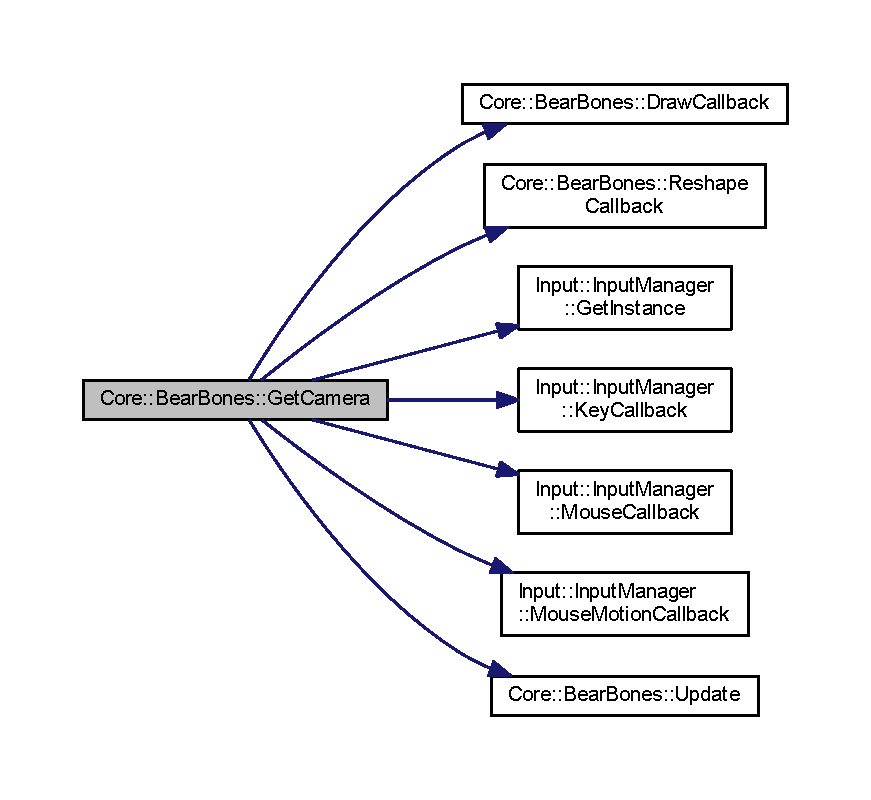
\includegraphics[width=350pt]{class_core_1_1_bear_bones_a4566808b082431ab19831dee7afd700b_cgraph}
\end{center}
\end{figure}
\mbox{\Hypertarget{class_core_1_1_bear_bones_acd30744bc23c254b1c211b3370c5285b}\label{class_core_1_1_bear_bones_acd30744bc23c254b1c211b3370c5285b}} 
\index{Core\+::\+Bear\+Bones@{Core\+::\+Bear\+Bones}!Get\+Instance@{Get\+Instance}}
\index{Get\+Instance@{Get\+Instance}!Core\+::\+Bear\+Bones@{Core\+::\+Bear\+Bones}}
\subsubsection{\texorpdfstring{Get\+Instance()}{GetInstance()}}
{\footnotesize\ttfamily \hyperlink{class_core_1_1_bear_bones}{Core\+::\+Bear\+Bones} $\ast$ Core\+::\+Bear\+Bones\+::\+Get\+Instance (\begin{DoxyParamCaption}{ }\end{DoxyParamCaption})\hspace{0.3cm}{\ttfamily [static]}}

Gets the singleton instance of the \hyperlink{class_core_1_1_bear_bones}{Bear\+Bones} engine. \begin{DoxyReturn}{Returns}
A pointer to the instance. 
\end{DoxyReturn}


Definition at line 5 of file Bear\+Bones.\+cpp.

\mbox{\Hypertarget{class_core_1_1_bear_bones_adf0f0c14fc729a3c7ac51297430b824d}\label{class_core_1_1_bear_bones_adf0f0c14fc729a3c7ac51297430b824d}} 
\index{Core\+::\+Bear\+Bones@{Core\+::\+Bear\+Bones}!Get\+Resource\+Loader@{Get\+Resource\+Loader}}
\index{Get\+Resource\+Loader@{Get\+Resource\+Loader}!Core\+::\+Bear\+Bones@{Core\+::\+Bear\+Bones}}
\subsubsection{\texorpdfstring{Get\+Resource\+Loader()}{GetResourceLoader()}}
{\footnotesize\ttfamily void Core\+::\+Bear\+Bones\+::\+Get\+Resource\+Loader (\begin{DoxyParamCaption}\item[{std\+::shared\+\_\+ptr$<$ \hyperlink{class_objects_1_1_resource_loader}{Objects\+::\+Resource\+Loader} $>$ \&}]{loader }\end{DoxyParamCaption})}

Gets the resource loader used in the engine. 
\begin{DoxyParams}[1]{Parameters}
\mbox{\tt out}  & {\em loader} & A pointer to the resource loader \\
\hline
\end{DoxyParams}


Definition at line 121 of file Bear\+Bones.\+cpp.

\mbox{\Hypertarget{class_core_1_1_bear_bones_a369f24d6903dc2cfb5c766fbbfdcdfb8}\label{class_core_1_1_bear_bones_a369f24d6903dc2cfb5c766fbbfdcdfb8}} 
\index{Core\+::\+Bear\+Bones@{Core\+::\+Bear\+Bones}!Get\+Window\+Size@{Get\+Window\+Size}}
\index{Get\+Window\+Size@{Get\+Window\+Size}!Core\+::\+Bear\+Bones@{Core\+::\+Bear\+Bones}}
\subsubsection{\texorpdfstring{Get\+Window\+Size()}{GetWindowSize()}}
{\footnotesize\ttfamily void Core\+::\+Bear\+Bones\+::\+Get\+Window\+Size (\begin{DoxyParamCaption}\item[{int \&}]{x,  }\item[{int \&}]{y }\end{DoxyParamCaption})}

Gets the current window size. 
\begin{DoxyParams}[1]{Parameters}
\mbox{\tt out}  & {\em x} & The width of the window. \\
\hline
\mbox{\tt out}  & {\em y} & The height of the window. \\
\hline
\end{DoxyParams}


Definition at line 105 of file Bear\+Bones.\+cpp.

\mbox{\Hypertarget{class_core_1_1_bear_bones_af5f9add95ce3557aa9f045c55a61a760}\label{class_core_1_1_bear_bones_af5f9add95ce3557aa9f045c55a61a760}} 
\index{Core\+::\+Bear\+Bones@{Core\+::\+Bear\+Bones}!Get\+World@{Get\+World}}
\index{Get\+World@{Get\+World}!Core\+::\+Bear\+Bones@{Core\+::\+Bear\+Bones}}
\subsubsection{\texorpdfstring{Get\+World()}{GetWorld()}}
{\footnotesize\ttfamily void Core\+::\+Bear\+Bones\+::\+Get\+World (\begin{DoxyParamCaption}\item[{std\+::shared\+\_\+ptr$<$ \hyperlink{class_objects_1_1_world}{Objects\+::\+World} $>$ \&}]{world }\end{DoxyParamCaption})}

Gets the world objects for the engine. 
\begin{DoxyParams}[1]{Parameters}
\mbox{\tt out}  & {\em world} & A pointer to the world. \\
\hline
\end{DoxyParams}


Definition at line 126 of file Bear\+Bones.\+cpp.

\mbox{\Hypertarget{class_core_1_1_bear_bones_a4023165c84d690ba6bade029bc60a710}\label{class_core_1_1_bear_bones_a4023165c84d690ba6bade029bc60a710}} 
\index{Core\+::\+Bear\+Bones@{Core\+::\+Bear\+Bones}!Initialize\+Window@{Initialize\+Window}}
\index{Initialize\+Window@{Initialize\+Window}!Core\+::\+Bear\+Bones@{Core\+::\+Bear\+Bones}}
\subsubsection{\texorpdfstring{Initialize\+Window()}{InitializeWindow()}}
{\footnotesize\ttfamily int Core\+::\+Bear\+Bones\+::\+Initialize\+Window (\begin{DoxyParamCaption}\item[{int $\ast$}]{argc,  }\item[{char $\ast$$\ast$}]{argv,  }\item[{int}]{winX,  }\item[{int}]{winY }\end{DoxyParamCaption})}

Initializes the engine. Will create the window and sets the size. 
\begin{DoxyParams}[1]{Parameters}
\mbox{\tt in,out}  & {\em argc} & The amount of input arguments, supplied from main. \\
\hline
\mbox{\tt in,out}  & {\em argv} & The input argument array. \\
\hline
\mbox{\tt in}  & {\em winX} & The width of the window. \\
\hline
\mbox{\tt in}  & {\em winY} & The height of the window. \\
\hline
\end{DoxyParams}


Definition at line 29 of file Bear\+Bones.\+cpp.

\mbox{\Hypertarget{class_core_1_1_bear_bones_a3e5b6f1994fdf8db744aba2f5a7547be}\label{class_core_1_1_bear_bones_a3e5b6f1994fdf8db744aba2f5a7547be}} 
\index{Core\+::\+Bear\+Bones@{Core\+::\+Bear\+Bones}!Quit@{Quit}}
\index{Quit@{Quit}!Core\+::\+Bear\+Bones@{Core\+::\+Bear\+Bones}}
\subsubsection{\texorpdfstring{Quit()}{Quit()}}
{\footnotesize\ttfamily void Core\+::\+Bear\+Bones\+::\+Quit (\begin{DoxyParamCaption}{ }\end{DoxyParamCaption})}

Closes and destroys the engine. 

Definition at line 111 of file Bear\+Bones.\+cpp.

\mbox{\Hypertarget{class_core_1_1_bear_bones_ad8ec7ea2b2e127f30fee7646359208e8}\label{class_core_1_1_bear_bones_ad8ec7ea2b2e127f30fee7646359208e8}} 
\index{Core\+::\+Bear\+Bones@{Core\+::\+Bear\+Bones}!Reshape\+Callback@{Reshape\+Callback}}
\index{Reshape\+Callback@{Reshape\+Callback}!Core\+::\+Bear\+Bones@{Core\+::\+Bear\+Bones}}
\subsubsection{\texorpdfstring{Reshape\+Callback()}{ReshapeCallback()}}
{\footnotesize\ttfamily void Core\+::\+Bear\+Bones\+::\+Reshape\+Callback (\begin{DoxyParamCaption}\item[{int}]{x,  }\item[{int}]{y }\end{DoxyParamCaption})}

The reshape callback. Called internally \begin{DoxyRefDesc}{Todo}
\item[\hyperlink{todo__todo000002}{Todo}]Make private \end{DoxyRefDesc}


Definition at line 87 of file Bear\+Bones.\+cpp.

Here is the caller graph for this function\+:
\nopagebreak
\begin{figure}[H]
\begin{center}
\leavevmode
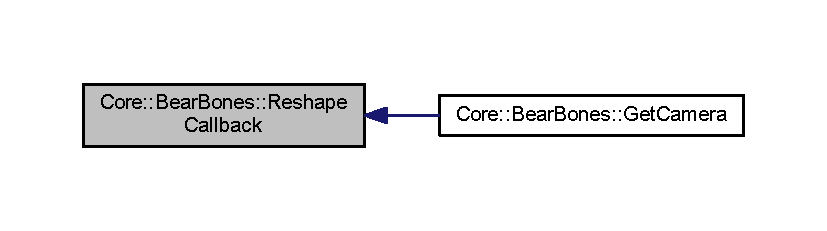
\includegraphics[width=350pt]{class_core_1_1_bear_bones_ad8ec7ea2b2e127f30fee7646359208e8_icgraph}
\end{center}
\end{figure}
\mbox{\Hypertarget{class_core_1_1_bear_bones_a980bca579db7dfbaebe2e8636660d0e2}\label{class_core_1_1_bear_bones_a980bca579db7dfbaebe2e8636660d0e2}} 
\index{Core\+::\+Bear\+Bones@{Core\+::\+Bear\+Bones}!Set\+Update\+Callback@{Set\+Update\+Callback}}
\index{Set\+Update\+Callback@{Set\+Update\+Callback}!Core\+::\+Bear\+Bones@{Core\+::\+Bear\+Bones}}
\subsubsection{\texorpdfstring{Set\+Update\+Callback()}{SetUpdateCallback()}}
{\footnotesize\ttfamily void Core\+::\+Bear\+Bones\+::\+Set\+Update\+Callback (\begin{DoxyParamCaption}\item[{f}]{callback }\end{DoxyParamCaption})}

Sets the update callback to call every frame. 
\begin{DoxyParams}{Parameters}
{\em callback} & A function pointer for the callback. \\
\hline
\end{DoxyParams}


Definition at line 116 of file Bear\+Bones.\+cpp.

\mbox{\Hypertarget{class_core_1_1_bear_bones_a5d424aa025bfbefd266e7777c657ebd9}\label{class_core_1_1_bear_bones_a5d424aa025bfbefd266e7777c657ebd9}} 
\index{Core\+::\+Bear\+Bones@{Core\+::\+Bear\+Bones}!Update@{Update}}
\index{Update@{Update}!Core\+::\+Bear\+Bones@{Core\+::\+Bear\+Bones}}
\subsubsection{\texorpdfstring{Update()}{Update()}}
{\footnotesize\ttfamily void Core\+::\+Bear\+Bones\+::\+Update (\begin{DoxyParamCaption}\item[{int}]{dx }\end{DoxyParamCaption})}

The internal update function 
\begin{DoxyParams}[1]{Parameters}
\mbox{\tt in}  & {\em dx} & The delta time. \\
\hline
\end{DoxyParams}
\begin{DoxyRefDesc}{Todo}
\item[\hyperlink{todo__todo000003}{Todo}]Make private. \end{DoxyRefDesc}


Definition at line 95 of file Bear\+Bones.\+cpp.

Here is the caller graph for this function\+:
\nopagebreak
\begin{figure}[H]
\begin{center}
\leavevmode
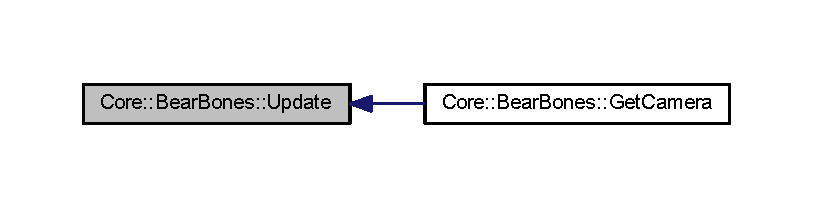
\includegraphics[width=350pt]{class_core_1_1_bear_bones_a5d424aa025bfbefd266e7777c657ebd9_icgraph}
\end{center}
\end{figure}


The documentation for this class was generated from the following files\+:\begin{DoxyCompactItemize}
\item 
Bear\+Bones-\/master/\+Bear\+Bones/src/\+Core/Bear\+Bones.\+h\item 
Bear\+Bones-\/master/\+Bear\+Bones/src/\+Core/Bear\+Bones.\+cpp\end{DoxyCompactItemize}

\hypertarget{class_objects_1_1_camera}{}\section{Objects\+:\+:Camera Class Reference}
\label{class_objects_1_1_camera}\index{Objects\+::\+Camera@{Objects\+::\+Camera}}


{\ttfamily \#include $<$Camera.\+h$>$}

\subsection*{Public Member Functions}
\begin{DoxyCompactItemize}
\item 
\mbox{\Hypertarget{class_objects_1_1_camera_ac3d1d2630c776a0925e1023cdf3cc11d}\label{class_objects_1_1_camera_ac3d1d2630c776a0925e1023cdf3cc11d}} 
{\bfseries Camera} (const \hyperlink{class_objects_1_1_camera}{Camera} \&other)
\item 
glm\+::vec3 \hyperlink{class_objects_1_1_camera_a8296a922839ed2ce11625d4062fdc00b}{Get\+Position} ()
\item 
float \hyperlink{class_objects_1_1_camera_a8febc4d7efdd0026ea17348bc64a9c0d}{Get\+Pitch} ()
\item 
float \hyperlink{class_objects_1_1_camera_a9af8c41d0824a875f650a8bcce6047f5}{Get\+Yaw} ()
\item 
float \hyperlink{class_objects_1_1_camera_a03d47a22c8591b487f11d30cff16323b}{Get\+Roll} ()
\item 
float \hyperlink{class_objects_1_1_camera_a9a84a8e6975b39d4f7c7b9826570b329}{Get\+Hover\+Height} ()
\item 
void \hyperlink{class_objects_1_1_camera_abf6ffbfbcdec52ecc9dbca948e8587cb}{Set\+Position} (glm\+::vec3 position)
\item 
void \hyperlink{class_objects_1_1_camera_aff13b2394968f618ace6caa6733bb672}{Set\+Position} (float x, float y, float z)
\item 
void \hyperlink{class_objects_1_1_camera_abcdee889581a7c03c751d091f3b5ea76}{Walk} (Camera\+Direction direction, int dt)
\item 
void \hyperlink{class_objects_1_1_camera_af74a18829347232af29cde68a3899331}{Strafe} (Camera\+Direction direction, int dt)
\item 
void \hyperlink{class_objects_1_1_camera_a08e2bef0b17c237525c9e8ad1695887b}{Rotate} (int dx, int dy, int dt)
\end{DoxyCompactItemize}


\subsection{Detailed Description}
A first person camera. Contains the positional and rotational data about the camera. \begin{DoxyAuthor}{Author}
Mathew Causby 
\end{DoxyAuthor}
\begin{DoxyVersion}{Version}
0.\+1 
\end{DoxyVersion}


Definition at line 25 of file Camera.\+h.



\subsection{Member Function Documentation}
\mbox{\Hypertarget{class_objects_1_1_camera_a9a84a8e6975b39d4f7c7b9826570b329}\label{class_objects_1_1_camera_a9a84a8e6975b39d4f7c7b9826570b329}} 
\index{Objects\+::\+Camera@{Objects\+::\+Camera}!Get\+Hover\+Height@{Get\+Hover\+Height}}
\index{Get\+Hover\+Height@{Get\+Hover\+Height}!Objects\+::\+Camera@{Objects\+::\+Camera}}
\subsubsection{\texorpdfstring{Get\+Hover\+Height()}{GetHoverHeight()}}
{\footnotesize\ttfamily float Objects\+::\+Camera\+::\+Get\+Hover\+Height (\begin{DoxyParamCaption}{ }\end{DoxyParamCaption})}

Gets the hover height of the camera. \begin{DoxyReturn}{Returns}
The hover height. 
\end{DoxyReturn}


Definition at line 49 of file Camera.\+cpp.

\mbox{\Hypertarget{class_objects_1_1_camera_a8febc4d7efdd0026ea17348bc64a9c0d}\label{class_objects_1_1_camera_a8febc4d7efdd0026ea17348bc64a9c0d}} 
\index{Objects\+::\+Camera@{Objects\+::\+Camera}!Get\+Pitch@{Get\+Pitch}}
\index{Get\+Pitch@{Get\+Pitch}!Objects\+::\+Camera@{Objects\+::\+Camera}}
\subsubsection{\texorpdfstring{Get\+Pitch()}{GetPitch()}}
{\footnotesize\ttfamily float Objects\+::\+Camera\+::\+Get\+Pitch (\begin{DoxyParamCaption}{ }\end{DoxyParamCaption})}

Gets the pitch of the camera. \begin{DoxyReturn}{Returns}
The pitch of the camera. 
\end{DoxyReturn}
\begin{DoxyNote}{Note}
Pitch represents the Y axis rotation 
\end{DoxyNote}


Definition at line 34 of file Camera.\+cpp.

\mbox{\Hypertarget{class_objects_1_1_camera_a8296a922839ed2ce11625d4062fdc00b}\label{class_objects_1_1_camera_a8296a922839ed2ce11625d4062fdc00b}} 
\index{Objects\+::\+Camera@{Objects\+::\+Camera}!Get\+Position@{Get\+Position}}
\index{Get\+Position@{Get\+Position}!Objects\+::\+Camera@{Objects\+::\+Camera}}
\subsubsection{\texorpdfstring{Get\+Position()}{GetPosition()}}
{\footnotesize\ttfamily glm\+::vec3 Objects\+::\+Camera\+::\+Get\+Position (\begin{DoxyParamCaption}{ }\end{DoxyParamCaption})}

Gets the current position of the camera. \begin{DoxyReturn}{Returns}
The position of the camera. 
\end{DoxyReturn}


Definition at line 29 of file Camera.\+cpp.

\mbox{\Hypertarget{class_objects_1_1_camera_a03d47a22c8591b487f11d30cff16323b}\label{class_objects_1_1_camera_a03d47a22c8591b487f11d30cff16323b}} 
\index{Objects\+::\+Camera@{Objects\+::\+Camera}!Get\+Roll@{Get\+Roll}}
\index{Get\+Roll@{Get\+Roll}!Objects\+::\+Camera@{Objects\+::\+Camera}}
\subsubsection{\texorpdfstring{Get\+Roll()}{GetRoll()}}
{\footnotesize\ttfamily float Objects\+::\+Camera\+::\+Get\+Roll (\begin{DoxyParamCaption}{ }\end{DoxyParamCaption})}

Gets the roll of the camera. \begin{DoxyReturn}{Returns}
The roll of the camera. 
\end{DoxyReturn}
\begin{DoxyNote}{Note}
Roll represents the X axis rotation. 
\end{DoxyNote}


Definition at line 44 of file Camera.\+cpp.

\mbox{\Hypertarget{class_objects_1_1_camera_a9af8c41d0824a875f650a8bcce6047f5}\label{class_objects_1_1_camera_a9af8c41d0824a875f650a8bcce6047f5}} 
\index{Objects\+::\+Camera@{Objects\+::\+Camera}!Get\+Yaw@{Get\+Yaw}}
\index{Get\+Yaw@{Get\+Yaw}!Objects\+::\+Camera@{Objects\+::\+Camera}}
\subsubsection{\texorpdfstring{Get\+Yaw()}{GetYaw()}}
{\footnotesize\ttfamily float Objects\+::\+Camera\+::\+Get\+Yaw (\begin{DoxyParamCaption}{ }\end{DoxyParamCaption})}

Gets the yaw of the camera. \begin{DoxyReturn}{Returns}
The yaw of the camera. 
\end{DoxyReturn}
\begin{DoxyNote}{Note}
Yaw represents the Z axis rotation 
\end{DoxyNote}


Definition at line 39 of file Camera.\+cpp.

\mbox{\Hypertarget{class_objects_1_1_camera_a08e2bef0b17c237525c9e8ad1695887b}\label{class_objects_1_1_camera_a08e2bef0b17c237525c9e8ad1695887b}} 
\index{Objects\+::\+Camera@{Objects\+::\+Camera}!Rotate@{Rotate}}
\index{Rotate@{Rotate}!Objects\+::\+Camera@{Objects\+::\+Camera}}
\subsubsection{\texorpdfstring{Rotate()}{Rotate()}}
{\footnotesize\ttfamily void Objects\+::\+Camera\+::\+Rotate (\begin{DoxyParamCaption}\item[{int}]{dx,  }\item[{int}]{dy,  }\item[{int}]{dt }\end{DoxyParamCaption})}

Rotates the camera by certain values. 
\begin{DoxyParams}[1]{Parameters}
\mbox{\tt in}  & {\em dx} & The change in x. \\
\hline
\mbox{\tt in}  & {\em dy} & The change in y. \\
\hline
\mbox{\tt in}  & {\em dt} & The delta time, provided in the update. \\
\hline
\end{DoxyParams}


Definition at line 94 of file Camera.\+cpp.

\mbox{\Hypertarget{class_objects_1_1_camera_abf6ffbfbcdec52ecc9dbca948e8587cb}\label{class_objects_1_1_camera_abf6ffbfbcdec52ecc9dbca948e8587cb}} 
\index{Objects\+::\+Camera@{Objects\+::\+Camera}!Set\+Position@{Set\+Position}}
\index{Set\+Position@{Set\+Position}!Objects\+::\+Camera@{Objects\+::\+Camera}}
\subsubsection{\texorpdfstring{Set\+Position()}{SetPosition()}\hspace{0.1cm}{\footnotesize\ttfamily [1/2]}}
{\footnotesize\ttfamily void Objects\+::\+Camera\+::\+Set\+Position (\begin{DoxyParamCaption}\item[{glm\+::vec3}]{position }\end{DoxyParamCaption})}

Sets the position of the camera. 
\begin{DoxyParams}[1]{Parameters}
\mbox{\tt in}  & {\em position} & The position of the camera. \\
\hline
\end{DoxyParams}


Definition at line 54 of file Camera.\+cpp.

\mbox{\Hypertarget{class_objects_1_1_camera_aff13b2394968f618ace6caa6733bb672}\label{class_objects_1_1_camera_aff13b2394968f618ace6caa6733bb672}} 
\index{Objects\+::\+Camera@{Objects\+::\+Camera}!Set\+Position@{Set\+Position}}
\index{Set\+Position@{Set\+Position}!Objects\+::\+Camera@{Objects\+::\+Camera}}
\subsubsection{\texorpdfstring{Set\+Position()}{SetPosition()}\hspace{0.1cm}{\footnotesize\ttfamily [2/2]}}
{\footnotesize\ttfamily void Objects\+::\+Camera\+::\+Set\+Position (\begin{DoxyParamCaption}\item[{float}]{x,  }\item[{float}]{y,  }\item[{float}]{z }\end{DoxyParamCaption})}

Sets the position of the camera. 
\begin{DoxyParams}[1]{Parameters}
\mbox{\tt in}  & {\em x} & The x position to set the camera to. \\
\hline
\mbox{\tt in}  & {\em y} & The y position to set the camera to. \\
\hline
\mbox{\tt in}  & {\em z} & The z position to set the camera to. \\
\hline
\end{DoxyParams}


Definition at line 59 of file Camera.\+cpp.

\mbox{\Hypertarget{class_objects_1_1_camera_af74a18829347232af29cde68a3899331}\label{class_objects_1_1_camera_af74a18829347232af29cde68a3899331}} 
\index{Objects\+::\+Camera@{Objects\+::\+Camera}!Strafe@{Strafe}}
\index{Strafe@{Strafe}!Objects\+::\+Camera@{Objects\+::\+Camera}}
\subsubsection{\texorpdfstring{Strafe()}{Strafe()}}
{\footnotesize\ttfamily void Objects\+::\+Camera\+::\+Strafe (\begin{DoxyParamCaption}\item[{Camera\+Direction}]{direction,  }\item[{int}]{dt }\end{DoxyParamCaption})}

Makes the camera strafe in a certain direction. Can be L\+E\+FT or R\+I\+G\+HT. 
\begin{DoxyParams}[1]{Parameters}
\mbox{\tt in}  & {\em direction} & The direction to strafe in. \\
\hline
\mbox{\tt in}  & {\em dt} & The delta time, provided in the update. \\
\hline
\end{DoxyParams}


Definition at line 80 of file Camera.\+cpp.

\mbox{\Hypertarget{class_objects_1_1_camera_abcdee889581a7c03c751d091f3b5ea76}\label{class_objects_1_1_camera_abcdee889581a7c03c751d091f3b5ea76}} 
\index{Objects\+::\+Camera@{Objects\+::\+Camera}!Walk@{Walk}}
\index{Walk@{Walk}!Objects\+::\+Camera@{Objects\+::\+Camera}}
\subsubsection{\texorpdfstring{Walk()}{Walk()}}
{\footnotesize\ttfamily void Objects\+::\+Camera\+::\+Walk (\begin{DoxyParamCaption}\item[{Camera\+Direction}]{direction,  }\item[{int}]{dt }\end{DoxyParamCaption})}

Makes the camera walk in a certain direction. Can be F\+O\+R\+W\+A\+RD or B\+A\+C\+K\+W\+A\+RD. 
\begin{DoxyParams}[1]{Parameters}
\mbox{\tt in}  & {\em direction} & The direction of to walk in. \\
\hline
\mbox{\tt in}  & {\em dt} & The delta time, provided in the update. \\
\hline
\end{DoxyParams}


Definition at line 66 of file Camera.\+cpp.



The documentation for this class was generated from the following files\+:\begin{DoxyCompactItemize}
\item 
Bear\+Bones-\/master/\+Bear\+Bones/src/\+Objects/Camera.\+h\item 
Bear\+Bones-\/master/\+Bear\+Bones/src/\+Objects/Camera.\+cpp\end{DoxyCompactItemize}

\hypertarget{class_objects_1_1_entity}{}\section{Objects\+:\+:Entity Class Reference}
\label{class_objects_1_1_entity}\index{Objects\+::\+Entity@{Objects\+::\+Entity}}


{\ttfamily \#include $<$Entity.\+h$>$}



Inheritance diagram for Objects\+:\+:Entity\+:
\nopagebreak
\begin{figure}[H]
\begin{center}
\leavevmode
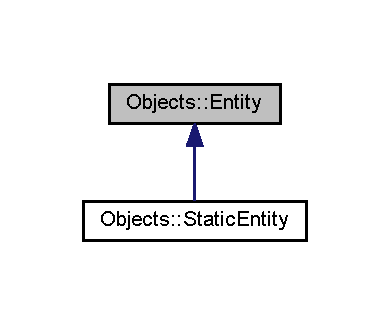
\includegraphics[width=187pt]{class_objects_1_1_entity__inherit__graph}
\end{center}
\end{figure}
\subsection*{Public Member Functions}
\begin{DoxyCompactItemize}
\item 
\mbox{\Hypertarget{class_objects_1_1_entity_ac432b784f855810ccba93d2e0168fedf}\label{class_objects_1_1_entity_ac432b784f855810ccba93d2e0168fedf}} 
{\bfseries Entity} (const \hyperlink{class_objects_1_1_entity}{Entity} \&other)
\item 
void \hyperlink{class_objects_1_1_entity_a1c4c5744e19cf3c201af92c390c492c4}{Set\+Model} (std\+::shared\+\_\+ptr$<$ \hyperlink{class_objects_1_1_obj_model}{Objects\+::\+Obj\+Model} $>$ model)
\item 
void \hyperlink{class_objects_1_1_entity_a53612458c6bd047cbf89d4ee8bcfdf91}{Set\+Position} (glm\+::vec3 position)
\item 
void \hyperlink{class_objects_1_1_entity_a26e73e8b7f3ed5b3583b14ccba2fd459}{Set\+Rotation} (glm\+::vec3 rotation)
\item 
void \hyperlink{class_objects_1_1_entity_af1cd8b1f5688d01647df4e5ea1d415ae}{Set\+Scale} (glm\+::vec3 scale)
\item 
std\+::shared\+\_\+ptr$<$ \hyperlink{class_objects_1_1_obj_model}{Objects\+::\+Obj\+Model} $>$ \hyperlink{class_objects_1_1_entity_ab11c284129ded400940d924965c70399}{Get\+Model} ()
\item 
glm\+::vec3 \hyperlink{class_objects_1_1_entity_a5ee0431c29c1912dcd6c1607fa051b74}{Get\+Position} ()
\item 
glm\+::vec3 \hyperlink{class_objects_1_1_entity_af859452e323ac3340ad7ac8f74bd6682}{Get\+Rotation} ()
\item 
glm\+::vec3 \hyperlink{class_objects_1_1_entity_accdd401dc7d81b86f1c56e0eba8e515b}{Get\+Scale} ()
\item 
virtual void \hyperlink{class_objects_1_1_entity_a3fc51fcad3f731410589f7ab0e3dbe7e}{Create\+Bounding\+Box} ()=0
\end{DoxyCompactItemize}


\subsection{Detailed Description}
An abstract class that describes an entity. The entity allows multiple drawings of an object without having to load it in multiple times. \begin{DoxyAuthor}{Author}
Mathew Causby 
\end{DoxyAuthor}
\begin{DoxyVersion}{Version}
0.\+1 
\end{DoxyVersion}


Definition at line 17 of file Entity.\+h.



\subsection{Member Function Documentation}
\mbox{\Hypertarget{class_objects_1_1_entity_a3fc51fcad3f731410589f7ab0e3dbe7e}\label{class_objects_1_1_entity_a3fc51fcad3f731410589f7ab0e3dbe7e}} 
\index{Objects\+::\+Entity@{Objects\+::\+Entity}!Create\+Bounding\+Box@{Create\+Bounding\+Box}}
\index{Create\+Bounding\+Box@{Create\+Bounding\+Box}!Objects\+::\+Entity@{Objects\+::\+Entity}}
\subsubsection{\texorpdfstring{Create\+Bounding\+Box()}{CreateBoundingBox()}}
{\footnotesize\ttfamily virtual void Objects\+::\+Entity\+::\+Create\+Bounding\+Box (\begin{DoxyParamCaption}{ }\end{DoxyParamCaption})\hspace{0.3cm}{\ttfamily [pure virtual]}}

Pure virtual function. Creates the bounding box. As each type of entity will have its own type of the bounding box. 

Implemented in \hyperlink{class_objects_1_1_static_entity_ae4b1ecdb50494a6d784b81803041ed52}{Objects\+::\+Static\+Entity}.

\mbox{\Hypertarget{class_objects_1_1_entity_ab11c284129ded400940d924965c70399}\label{class_objects_1_1_entity_ab11c284129ded400940d924965c70399}} 
\index{Objects\+::\+Entity@{Objects\+::\+Entity}!Get\+Model@{Get\+Model}}
\index{Get\+Model@{Get\+Model}!Objects\+::\+Entity@{Objects\+::\+Entity}}
\subsubsection{\texorpdfstring{Get\+Model()}{GetModel()}}
{\footnotesize\ttfamily std\+::shared\+\_\+ptr$<$ \hyperlink{class_objects_1_1_obj_model}{Objects\+::\+Obj\+Model} $>$ Objects\+::\+Entity\+::\+Get\+Model (\begin{DoxyParamCaption}{ }\end{DoxyParamCaption})}

Gets a shared pointer to the model to draw. \begin{DoxyReturn}{Returns}
The pointer to the model. 
\end{DoxyReturn}


Definition at line 43 of file Entity.\+cpp.

\mbox{\Hypertarget{class_objects_1_1_entity_a5ee0431c29c1912dcd6c1607fa051b74}\label{class_objects_1_1_entity_a5ee0431c29c1912dcd6c1607fa051b74}} 
\index{Objects\+::\+Entity@{Objects\+::\+Entity}!Get\+Position@{Get\+Position}}
\index{Get\+Position@{Get\+Position}!Objects\+::\+Entity@{Objects\+::\+Entity}}
\subsubsection{\texorpdfstring{Get\+Position()}{GetPosition()}}
{\footnotesize\ttfamily glm\+::vec3 Objects\+::\+Entity\+::\+Get\+Position (\begin{DoxyParamCaption}{ }\end{DoxyParamCaption})}

Gets the position of the entity. \begin{DoxyReturn}{Returns}
The position of the entity. 
\end{DoxyReturn}


Definition at line 48 of file Entity.\+cpp.

\mbox{\Hypertarget{class_objects_1_1_entity_af859452e323ac3340ad7ac8f74bd6682}\label{class_objects_1_1_entity_af859452e323ac3340ad7ac8f74bd6682}} 
\index{Objects\+::\+Entity@{Objects\+::\+Entity}!Get\+Rotation@{Get\+Rotation}}
\index{Get\+Rotation@{Get\+Rotation}!Objects\+::\+Entity@{Objects\+::\+Entity}}
\subsubsection{\texorpdfstring{Get\+Rotation()}{GetRotation()}}
{\footnotesize\ttfamily glm\+::vec3 Objects\+::\+Entity\+::\+Get\+Rotation (\begin{DoxyParamCaption}{ }\end{DoxyParamCaption})}

Gets the rotation of the entity. \begin{DoxyReturn}{Returns}
The rotation of the entity. 
\end{DoxyReturn}


Definition at line 53 of file Entity.\+cpp.

\mbox{\Hypertarget{class_objects_1_1_entity_accdd401dc7d81b86f1c56e0eba8e515b}\label{class_objects_1_1_entity_accdd401dc7d81b86f1c56e0eba8e515b}} 
\index{Objects\+::\+Entity@{Objects\+::\+Entity}!Get\+Scale@{Get\+Scale}}
\index{Get\+Scale@{Get\+Scale}!Objects\+::\+Entity@{Objects\+::\+Entity}}
\subsubsection{\texorpdfstring{Get\+Scale()}{GetScale()}}
{\footnotesize\ttfamily glm\+::vec3 Objects\+::\+Entity\+::\+Get\+Scale (\begin{DoxyParamCaption}{ }\end{DoxyParamCaption})}

Gets the scale of the entity. \begin{DoxyReturn}{Returns}
The scale of the entity. 
\end{DoxyReturn}


Definition at line 58 of file Entity.\+cpp.

\mbox{\Hypertarget{class_objects_1_1_entity_a1c4c5744e19cf3c201af92c390c492c4}\label{class_objects_1_1_entity_a1c4c5744e19cf3c201af92c390c492c4}} 
\index{Objects\+::\+Entity@{Objects\+::\+Entity}!Set\+Model@{Set\+Model}}
\index{Set\+Model@{Set\+Model}!Objects\+::\+Entity@{Objects\+::\+Entity}}
\subsubsection{\texorpdfstring{Set\+Model()}{SetModel()}}
{\footnotesize\ttfamily void Objects\+::\+Entity\+::\+Set\+Model (\begin{DoxyParamCaption}\item[{std\+::shared\+\_\+ptr$<$ \hyperlink{class_objects_1_1_obj_model}{Objects\+::\+Obj\+Model} $>$}]{model }\end{DoxyParamCaption})}

Sets the model of the entity. 
\begin{DoxyParams}[1]{Parameters}
\mbox{\tt in}  & {\em model} & A shared pointer to the model. \\
\hline
\end{DoxyParams}


Definition at line 23 of file Entity.\+cpp.

\mbox{\Hypertarget{class_objects_1_1_entity_a53612458c6bd047cbf89d4ee8bcfdf91}\label{class_objects_1_1_entity_a53612458c6bd047cbf89d4ee8bcfdf91}} 
\index{Objects\+::\+Entity@{Objects\+::\+Entity}!Set\+Position@{Set\+Position}}
\index{Set\+Position@{Set\+Position}!Objects\+::\+Entity@{Objects\+::\+Entity}}
\subsubsection{\texorpdfstring{Set\+Position()}{SetPosition()}}
{\footnotesize\ttfamily void Objects\+::\+Entity\+::\+Set\+Position (\begin{DoxyParamCaption}\item[{glm\+::vec3}]{position }\end{DoxyParamCaption})}

Sets the position of the entity. 
\begin{DoxyParams}[1]{Parameters}
\mbox{\tt in}  & {\em position} & The position of the entity \\
\hline
\end{DoxyParams}


Definition at line 28 of file Entity.\+cpp.

\mbox{\Hypertarget{class_objects_1_1_entity_a26e73e8b7f3ed5b3583b14ccba2fd459}\label{class_objects_1_1_entity_a26e73e8b7f3ed5b3583b14ccba2fd459}} 
\index{Objects\+::\+Entity@{Objects\+::\+Entity}!Set\+Rotation@{Set\+Rotation}}
\index{Set\+Rotation@{Set\+Rotation}!Objects\+::\+Entity@{Objects\+::\+Entity}}
\subsubsection{\texorpdfstring{Set\+Rotation()}{SetRotation()}}
{\footnotesize\ttfamily void Objects\+::\+Entity\+::\+Set\+Rotation (\begin{DoxyParamCaption}\item[{glm\+::vec3}]{rotation }\end{DoxyParamCaption})}

Sets the rotation of the entity. 
\begin{DoxyParams}[1]{Parameters}
\mbox{\tt in}  & {\em rotation} & The rotation of the entity. \\
\hline
\end{DoxyParams}


Definition at line 33 of file Entity.\+cpp.

\mbox{\Hypertarget{class_objects_1_1_entity_af1cd8b1f5688d01647df4e5ea1d415ae}\label{class_objects_1_1_entity_af1cd8b1f5688d01647df4e5ea1d415ae}} 
\index{Objects\+::\+Entity@{Objects\+::\+Entity}!Set\+Scale@{Set\+Scale}}
\index{Set\+Scale@{Set\+Scale}!Objects\+::\+Entity@{Objects\+::\+Entity}}
\subsubsection{\texorpdfstring{Set\+Scale()}{SetScale()}}
{\footnotesize\ttfamily void Objects\+::\+Entity\+::\+Set\+Scale (\begin{DoxyParamCaption}\item[{glm\+::vec3}]{scale }\end{DoxyParamCaption})}

Sets the scale of the entity. 
\begin{DoxyParams}[1]{Parameters}
\mbox{\tt in}  & {\em scale} & The scale of the entity. \\
\hline
\end{DoxyParams}


Definition at line 38 of file Entity.\+cpp.



The documentation for this class was generated from the following files\+:\begin{DoxyCompactItemize}
\item 
Bear\+Bones-\/master/\+Bear\+Bones/src/\+Objects/Entity.\+h\item 
Bear\+Bones-\/master/\+Bear\+Bones/src/\+Objects/Entity.\+cpp\end{DoxyCompactItemize}

\hypertarget{class_input_1_1_input_manager}{}\section{Input\+:\+:Input\+Manager Class Reference}
\label{class_input_1_1_input_manager}\index{Input\+::\+Input\+Manager@{Input\+::\+Input\+Manager}}


{\ttfamily \#include $<$Input\+Manager.\+h$>$}

\subsection*{Public Member Functions}
\begin{DoxyCompactItemize}
\item 
Key\+State \hyperlink{class_input_1_1_input_manager_a6ac7c060e63c0f30563c29b9d2b41476}{Get\+Key\+State} (int key)
\item 
void \hyperlink{class_input_1_1_input_manager_abb16770c5d1d69326dbe931782a5c0e5}{Get\+Mouse\+Position} (int \&x, int \&y)
\item 
Button\+State \hyperlink{class_input_1_1_input_manager_a42a6d92229690b8dc363dbf3012d20e1}{Get\+Button\+State} (int button)
\item 
void \hyperlink{class_input_1_1_input_manager_a81353902fe615c99f742cd280335e72f}{Key\+Callback} (int key, bool pressed)
\item 
void \hyperlink{class_input_1_1_input_manager_a9ec4f960256ab6a8b50297b9e3bf0307}{Mouse\+Callback} (int button, int state, int x, int y)
\item 
void \hyperlink{class_input_1_1_input_manager_ab241c84c47dd69505ea51e93a33f2113}{Mouse\+Motion\+Callback} (int x, int y)
\end{DoxyCompactItemize}
\subsection*{Static Public Member Functions}
\begin{DoxyCompactItemize}
\item 
static \hyperlink{class_input_1_1_input_manager}{Input\+Manager} $\ast$ \hyperlink{class_input_1_1_input_manager_ac4df9b50e7cfc4e59f061a08ed7f4925}{Get\+Instance} ()
\end{DoxyCompactItemize}


\subsection{Detailed Description}
The singleton class for managing the input for the engine. Stores the state of each mouse and keyboard to be polled at will. \begin{DoxyAuthor}{Author}
Mathew Causby 
\end{DoxyAuthor}
\begin{DoxyVersion}{Version}
0.\+1 
\end{DoxyVersion}


Definition at line 33 of file Input\+Manager.\+h.



\subsection{Member Function Documentation}
\mbox{\Hypertarget{class_input_1_1_input_manager_a42a6d92229690b8dc363dbf3012d20e1}\label{class_input_1_1_input_manager_a42a6d92229690b8dc363dbf3012d20e1}} 
\index{Input\+::\+Input\+Manager@{Input\+::\+Input\+Manager}!Get\+Button\+State@{Get\+Button\+State}}
\index{Get\+Button\+State@{Get\+Button\+State}!Input\+::\+Input\+Manager@{Input\+::\+Input\+Manager}}
\subsubsection{\texorpdfstring{Get\+Button\+State()}{GetButtonState()}}
{\footnotesize\ttfamily Input\+::\+Button\+State Input\+::\+Input\+Manager\+::\+Get\+Button\+State (\begin{DoxyParamCaption}\item[{int}]{button }\end{DoxyParamCaption})}

Gets the button state of the mouse. 
\begin{DoxyParams}[1]{Parameters}
\mbox{\tt in}  & {\em button} & The mouse button to check. \\
\hline
\end{DoxyParams}
\begin{DoxyReturn}{Returns}
The current state of the button. Will be B\+S\+\_\+\+B\+U\+T\+T\+O\+N\+\_\+\+C\+L\+I\+CK on first check, and it updates to B\+S\+\_\+\+B\+U\+T\+T\+O\+N\+\_\+\+D\+O\+WN for every subsequent check. 
\end{DoxyReturn}


Definition at line 51 of file Input\+Manager.\+cpp.

\mbox{\Hypertarget{class_input_1_1_input_manager_ac4df9b50e7cfc4e59f061a08ed7f4925}\label{class_input_1_1_input_manager_ac4df9b50e7cfc4e59f061a08ed7f4925}} 
\index{Input\+::\+Input\+Manager@{Input\+::\+Input\+Manager}!Get\+Instance@{Get\+Instance}}
\index{Get\+Instance@{Get\+Instance}!Input\+::\+Input\+Manager@{Input\+::\+Input\+Manager}}
\subsubsection{\texorpdfstring{Get\+Instance()}{GetInstance()}}
{\footnotesize\ttfamily \hyperlink{class_input_1_1_input_manager}{Input\+::\+Input\+Manager} $\ast$ Input\+::\+Input\+Manager\+::\+Get\+Instance (\begin{DoxyParamCaption}{ }\end{DoxyParamCaption})\hspace{0.3cm}{\ttfamily [static]}}

Gets the singleton instance of the input manager. \begin{DoxyReturn}{Returns}
A pointer to the \hyperlink{class_input_1_1_input_manager}{Input\+Manager} instance. 
\end{DoxyReturn}


Definition at line 28 of file Input\+Manager.\+cpp.

Here is the caller graph for this function\+:
\nopagebreak
\begin{figure}[H]
\begin{center}
\leavevmode
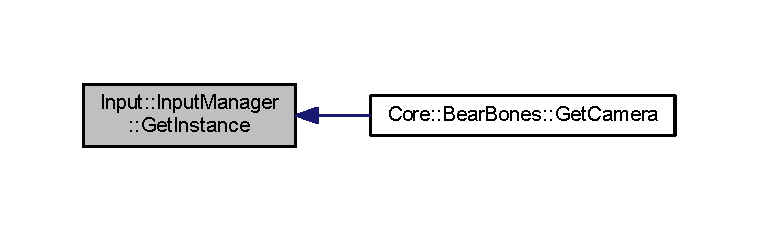
\includegraphics[width=350pt]{class_input_1_1_input_manager_ac4df9b50e7cfc4e59f061a08ed7f4925_icgraph}
\end{center}
\end{figure}
\mbox{\Hypertarget{class_input_1_1_input_manager_a6ac7c060e63c0f30563c29b9d2b41476}\label{class_input_1_1_input_manager_a6ac7c060e63c0f30563c29b9d2b41476}} 
\index{Input\+::\+Input\+Manager@{Input\+::\+Input\+Manager}!Get\+Key\+State@{Get\+Key\+State}}
\index{Get\+Key\+State@{Get\+Key\+State}!Input\+::\+Input\+Manager@{Input\+::\+Input\+Manager}}
\subsubsection{\texorpdfstring{Get\+Key\+State()}{GetKeyState()}}
{\footnotesize\ttfamily Input\+::\+Key\+State Input\+::\+Input\+Manager\+::\+Get\+Key\+State (\begin{DoxyParamCaption}\item[{int}]{key }\end{DoxyParamCaption})}

Gets the current key state of the key. 
\begin{DoxyParams}[1]{Parameters}
\mbox{\tt in}  & {\em key} & The key to check. \\
\hline
\end{DoxyParams}
\begin{DoxyReturn}{Returns}
The state of the key. Will be K\+S\+\_\+\+K\+E\+Y\+\_\+\+P\+R\+E\+S\+S\+ED on first check, then it updates to K\+S\+\_\+\+K\+E\+Y\+\_\+\+R\+E\+P\+E\+AT for every subsequent check. 
\end{DoxyReturn}
\begin{DoxyNote}{Note}
The key is an integer. Can pass a char in place and it will use the A\+S\+C\+II value automatically. 
\end{DoxyNote}


Definition at line 37 of file Input\+Manager.\+cpp.

\mbox{\Hypertarget{class_input_1_1_input_manager_abb16770c5d1d69326dbe931782a5c0e5}\label{class_input_1_1_input_manager_abb16770c5d1d69326dbe931782a5c0e5}} 
\index{Input\+::\+Input\+Manager@{Input\+::\+Input\+Manager}!Get\+Mouse\+Position@{Get\+Mouse\+Position}}
\index{Get\+Mouse\+Position@{Get\+Mouse\+Position}!Input\+::\+Input\+Manager@{Input\+::\+Input\+Manager}}
\subsubsection{\texorpdfstring{Get\+Mouse\+Position()}{GetMousePosition()}}
{\footnotesize\ttfamily void Input\+::\+Input\+Manager\+::\+Get\+Mouse\+Position (\begin{DoxyParamCaption}\item[{int \&}]{x,  }\item[{int \&}]{y }\end{DoxyParamCaption})}

Gets the mouse position. 
\begin{DoxyParams}[1]{Parameters}
\mbox{\tt out}  & {\em x} & The x position of the mouse. \\
\hline
\mbox{\tt out}  & {\em y} & The y position of the mouse. \\
\hline
\end{DoxyParams}


Definition at line 45 of file Input\+Manager.\+cpp.

\mbox{\Hypertarget{class_input_1_1_input_manager_a81353902fe615c99f742cd280335e72f}\label{class_input_1_1_input_manager_a81353902fe615c99f742cd280335e72f}} 
\index{Input\+::\+Input\+Manager@{Input\+::\+Input\+Manager}!Key\+Callback@{Key\+Callback}}
\index{Key\+Callback@{Key\+Callback}!Input\+::\+Input\+Manager@{Input\+::\+Input\+Manager}}
\subsubsection{\texorpdfstring{Key\+Callback()}{KeyCallback()}}
{\footnotesize\ttfamily void Input\+::\+Input\+Manager\+::\+Key\+Callback (\begin{DoxyParamCaption}\item[{int}]{key,  }\item[{bool}]{pressed }\end{DoxyParamCaption})}

The callback that will set the key internal values. 
\begin{DoxyParams}[1]{Parameters}
\mbox{\tt in}  & {\em key} & The key that recieved the event. \\
\hline
\mbox{\tt in}  & {\em pressed} & If the key has been pressed or not. \\
\hline
\end{DoxyParams}


Definition at line 59 of file Input\+Manager.\+cpp.

Here is the caller graph for this function\+:
\nopagebreak
\begin{figure}[H]
\begin{center}
\leavevmode
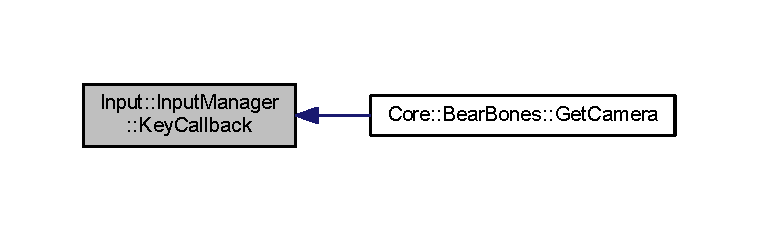
\includegraphics[width=350pt]{class_input_1_1_input_manager_a81353902fe615c99f742cd280335e72f_icgraph}
\end{center}
\end{figure}
\mbox{\Hypertarget{class_input_1_1_input_manager_a9ec4f960256ab6a8b50297b9e3bf0307}\label{class_input_1_1_input_manager_a9ec4f960256ab6a8b50297b9e3bf0307}} 
\index{Input\+::\+Input\+Manager@{Input\+::\+Input\+Manager}!Mouse\+Callback@{Mouse\+Callback}}
\index{Mouse\+Callback@{Mouse\+Callback}!Input\+::\+Input\+Manager@{Input\+::\+Input\+Manager}}
\subsubsection{\texorpdfstring{Mouse\+Callback()}{MouseCallback()}}
{\footnotesize\ttfamily void Input\+::\+Input\+Manager\+::\+Mouse\+Callback (\begin{DoxyParamCaption}\item[{int}]{button,  }\item[{int}]{state,  }\item[{int}]{x,  }\item[{int}]{y }\end{DoxyParamCaption})}

The callback that will set the mouse internal values. 
\begin{DoxyParams}[1]{Parameters}
\mbox{\tt in}  & {\em button} & The button that recieved the event. \\
\hline
\mbox{\tt in}  & {\em state} & The state of the button. \\
\hline
\mbox{\tt in}  & {\em x} & The x position of the mouse at the time of the event. \\
\hline
\mbox{\tt in}  & {\em y} & The y position of the mouse at the time of the event. \\
\hline
\end{DoxyParams}


Definition at line 66 of file Input\+Manager.\+cpp.

Here is the caller graph for this function\+:
\nopagebreak
\begin{figure}[H]
\begin{center}
\leavevmode
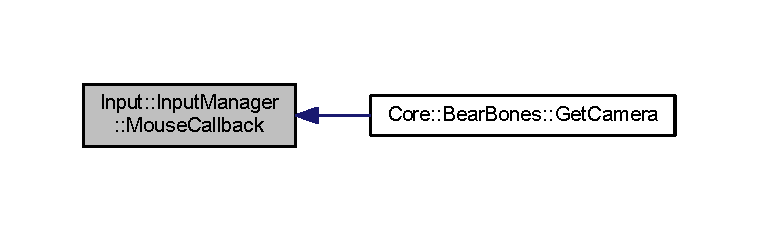
\includegraphics[width=350pt]{class_input_1_1_input_manager_a9ec4f960256ab6a8b50297b9e3bf0307_icgraph}
\end{center}
\end{figure}
\mbox{\Hypertarget{class_input_1_1_input_manager_ab241c84c47dd69505ea51e93a33f2113}\label{class_input_1_1_input_manager_ab241c84c47dd69505ea51e93a33f2113}} 
\index{Input\+::\+Input\+Manager@{Input\+::\+Input\+Manager}!Mouse\+Motion\+Callback@{Mouse\+Motion\+Callback}}
\index{Mouse\+Motion\+Callback@{Mouse\+Motion\+Callback}!Input\+::\+Input\+Manager@{Input\+::\+Input\+Manager}}
\subsubsection{\texorpdfstring{Mouse\+Motion\+Callback()}{MouseMotionCallback()}}
{\footnotesize\ttfamily void Input\+::\+Input\+Manager\+::\+Mouse\+Motion\+Callback (\begin{DoxyParamCaption}\item[{int}]{x,  }\item[{int}]{y }\end{DoxyParamCaption})}

The callback that will set the mouse position. 
\begin{DoxyParams}[1]{Parameters}
\mbox{\tt in}  & {\em x} & The x position of the mouse. \\
\hline
\mbox{\tt in}  & {\em y} & The y position of the mouse. \\
\hline
\end{DoxyParams}


Definition at line 73 of file Input\+Manager.\+cpp.

Here is the caller graph for this function\+:
\nopagebreak
\begin{figure}[H]
\begin{center}
\leavevmode
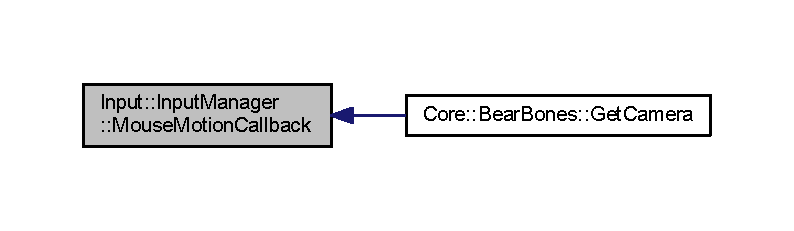
\includegraphics[width=350pt]{class_input_1_1_input_manager_ab241c84c47dd69505ea51e93a33f2113_icgraph}
\end{center}
\end{figure}


The documentation for this class was generated from the following files\+:\begin{DoxyCompactItemize}
\item 
Bear\+Bones-\/master/\+Bear\+Bones/src/\+Input/Input\+Manager.\+h\item 
Bear\+Bones-\/master/\+Bear\+Bones/src/\+Input/Input\+Manager.\+cpp\end{DoxyCompactItemize}

\hypertarget{class_util_1_1_math_util}{}\section{Util\+:\+:Math\+Util Class Reference}
\label{class_util_1_1_math_util}\index{Util\+::\+Math\+Util@{Util\+::\+Math\+Util}}


{\ttfamily \#include $<$Math\+Util.\+h$>$}

\subsection*{Static Public Member Functions}
\begin{DoxyCompactItemize}
\item 
static glm\+::mat4x4 \hyperlink{class_util_1_1_math_util_aecfa1962d61e7f63d30bee7dbeb0cd9f}{Get\+Transformation\+Matrix} (glm\+::vec3 translation, glm\+::vec3 rotation, glm\+::vec3 scale)
\item 
static glm\+::mat4x4 \hyperlink{class_util_1_1_math_util_abbc94837eaa9a0e2bb4c772a61b36ce7}{Get\+View\+Matrix} (float x, float y, float z, float pitch, float yaw, float roll)
\end{DoxyCompactItemize}


\subsection{Detailed Description}
Contains mathematical helper functions. \begin{DoxyAuthor}{Author}
Mathew Causby. 
\end{DoxyAuthor}
\begin{DoxyVersion}{Version}
0.\+1 
\end{DoxyVersion}


Definition at line 16 of file Math\+Util.\+h.



\subsection{Member Function Documentation}
\mbox{\Hypertarget{class_util_1_1_math_util_aecfa1962d61e7f63d30bee7dbeb0cd9f}\label{class_util_1_1_math_util_aecfa1962d61e7f63d30bee7dbeb0cd9f}} 
\index{Util\+::\+Math\+Util@{Util\+::\+Math\+Util}!Get\+Transformation\+Matrix@{Get\+Transformation\+Matrix}}
\index{Get\+Transformation\+Matrix@{Get\+Transformation\+Matrix}!Util\+::\+Math\+Util@{Util\+::\+Math\+Util}}
\subsubsection{\texorpdfstring{Get\+Transformation\+Matrix()}{GetTransformationMatrix()}}
{\footnotesize\ttfamily glm\+::mat4x4 Util\+::\+Math\+Util\+::\+Get\+Transformation\+Matrix (\begin{DoxyParamCaption}\item[{glm\+::vec3}]{translation,  }\item[{glm\+::vec3}]{rotation,  }\item[{glm\+::vec3}]{scale }\end{DoxyParamCaption})\hspace{0.3cm}{\ttfamily [static]}}

Creates and retrieves a transformation matrix. 
\begin{DoxyParams}[1]{Parameters}
\mbox{\tt in}  & {\em translation} & Where the object has moved to. \\
\hline
\mbox{\tt in}  & {\em rotation} & How the object has rotated. \\
\hline
\mbox{\tt in}  & {\em scale} & How the object is scaled. \\
\hline
\end{DoxyParams}
\begin{DoxyReturn}{Returns}
A matrix containing the translation, rotation, and scale transformationms. 
\end{DoxyReturn}


Definition at line 3 of file Math\+Util.\+cpp.

Here is the caller graph for this function\+:
\nopagebreak
\begin{figure}[H]
\begin{center}
\leavevmode
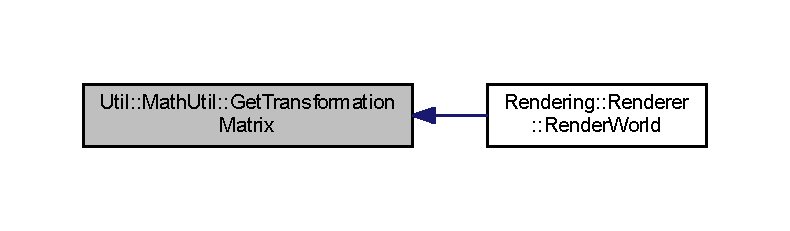
\includegraphics[width=350pt]{class_util_1_1_math_util_aecfa1962d61e7f63d30bee7dbeb0cd9f_icgraph}
\end{center}
\end{figure}
\mbox{\Hypertarget{class_util_1_1_math_util_abbc94837eaa9a0e2bb4c772a61b36ce7}\label{class_util_1_1_math_util_abbc94837eaa9a0e2bb4c772a61b36ce7}} 
\index{Util\+::\+Math\+Util@{Util\+::\+Math\+Util}!Get\+View\+Matrix@{Get\+View\+Matrix}}
\index{Get\+View\+Matrix@{Get\+View\+Matrix}!Util\+::\+Math\+Util@{Util\+::\+Math\+Util}}
\subsubsection{\texorpdfstring{Get\+View\+Matrix()}{GetViewMatrix()}}
{\footnotesize\ttfamily glm\+::mat4x4 Util\+::\+Math\+Util\+::\+Get\+View\+Matrix (\begin{DoxyParamCaption}\item[{float}]{x,  }\item[{float}]{y,  }\item[{float}]{z,  }\item[{float}]{pitch,  }\item[{float}]{yaw,  }\item[{float}]{roll }\end{DoxyParamCaption})\hspace{0.3cm}{\ttfamily [static]}}

Creates and retrieved a view matrix. View matrix being where the \char`\"{}camera\char`\"{} is 
\begin{DoxyParams}[1]{Parameters}
\mbox{\tt in}  & {\em x} & The x position \\
\hline
\mbox{\tt in}  & {\em y} & The y position \\
\hline
\mbox{\tt in}  & {\em z} & The z position \\
\hline
\mbox{\tt in}  & {\em pitch} & The pitch, or the y rotation. \\
\hline
\mbox{\tt in}  & {\em yaw} & The yaw, or the z rotation. \\
\hline
\mbox{\tt in}  & {\em roll} & The roll, or the x rotation. \\
\hline
\end{DoxyParams}
\begin{DoxyReturn}{Returns}
A matrix describing the transformation based on the camera. 
\end{DoxyReturn}


Definition at line 14 of file Math\+Util.\+cpp.

Here is the caller graph for this function\+:
\nopagebreak
\begin{figure}[H]
\begin{center}
\leavevmode
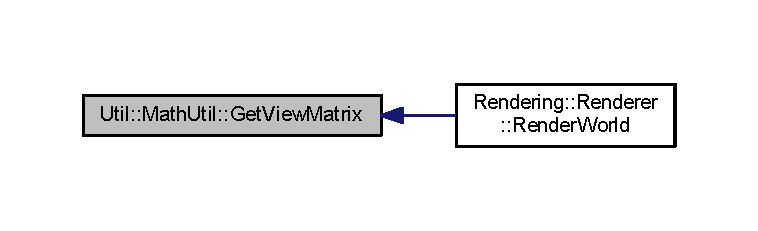
\includegraphics[width=350pt]{class_util_1_1_math_util_abbc94837eaa9a0e2bb4c772a61b36ce7_icgraph}
\end{center}
\end{figure}


The documentation for this class was generated from the following files\+:\begin{DoxyCompactItemize}
\item 
Bear\+Bones-\/master/\+Bear\+Bones/src/\+Util/Math\+Util.\+h\item 
Bear\+Bones-\/master/\+Bear\+Bones/src/\+Util/Math\+Util.\+cpp\end{DoxyCompactItemize}

\hypertarget{class_collision_1_1_o_b_b}{}\section{Collision\+:\+:O\+BB Class Reference}
\label{class_collision_1_1_o_b_b}\index{Collision\+::\+O\+BB@{Collision\+::\+O\+BB}}


{\ttfamily \#include $<$O\+B\+B.\+h$>$}

\subsection*{Public Member Functions}
\begin{DoxyCompactItemize}
\item 
\mbox{\Hypertarget{class_collision_1_1_o_b_b_a51cc3cb50610b7f71f35286b7279e864}\label{class_collision_1_1_o_b_b_a51cc3cb50610b7f71f35286b7279e864}} 
{\bfseries O\+BB} (const \hyperlink{class_collision_1_1_o_b_b}{O\+BB} \&other)
\end{DoxyCompactItemize}


\subsection{Detailed Description}
An Oriented Bounding Box. \begin{DoxyAuthor}{Author}
Mathew Causby 
\end{DoxyAuthor}
\begin{DoxyVersion}{Version}
0.\+1 
\end{DoxyVersion}


Definition at line 14 of file O\+B\+B.\+h.



The documentation for this class was generated from the following files\+:\begin{DoxyCompactItemize}
\item 
Bear\+Bones-\/master/\+Bear\+Bones/src/\+Collision/O\+B\+B.\+h\item 
Bear\+Bones-\/master/\+Bear\+Bones/src/\+Collision/O\+B\+B.\+cpp\end{DoxyCompactItemize}

\hypertarget{class_objects_1_1_obj_model}{}\section{Objects\+:\+:Obj\+Model Class Reference}
\label{class_objects_1_1_obj_model}\index{Objects\+::\+Obj\+Model@{Objects\+::\+Obj\+Model}}


{\ttfamily \#include $<$Obj\+Model.\+h$>$}

\subsection*{Public Member Functions}
\begin{DoxyCompactItemize}
\item 
\mbox{\Hypertarget{class_objects_1_1_obj_model_aa2d303c5c56929ba6a4ad241626f6c2f}\label{class_objects_1_1_obj_model_aa2d303c5c56929ba6a4ad241626f6c2f}} 
{\bfseries Obj\+Model} (const \hyperlink{class_objects_1_1_obj_model}{Obj\+Model} \&other)
\item 
void \hyperlink{class_objects_1_1_obj_model_a7a6747283cab7ded9bb454046bae15d7}{Set\+V\+A\+O\+ID} (int vao\+Id)
\item 
void \hyperlink{class_objects_1_1_obj_model_a863d5f8618de5bf3cc52de85181f178b}{Set\+Vertex\+Count} (int count)
\item 
void \hyperlink{class_objects_1_1_obj_model_a8dbe139248efa6ed1d9921e141262ee9}{Set\+Model\+Height} (double height)
\item 
void \hyperlink{class_objects_1_1_obj_model_a72ef59adfa1dd88840178aa76479e471}{Set\+Texture} (std\+::shared\+\_\+ptr$<$ \hyperlink{class_objects_1_1_texture}{Texture} $>$ tex)
\item 
void \hyperlink{class_objects_1_1_obj_model_aea0369b1cff1d80289d6378e8b98bc57}{Set\+Verticies} (std\+::vector$<$ glm\+::vec3 $>$ verts)
\item 
void \hyperlink{class_objects_1_1_obj_model_a33b342b503c772b35d8d8c557ec874b4}{Set\+U\+Vs} (std\+::vector$<$ glm\+::vec2 $>$ uvs)
\item 
void \hyperlink{class_objects_1_1_obj_model_aaa85b89c8fd001ad528a733483e1e7c9}{Set\+Normals} (std\+::vector$<$ glm\+::vec3 $>$ norms)
\item 
int \hyperlink{class_objects_1_1_obj_model_a197b62526db5e58e16e455bd6faf5da0}{Get\+V\+A\+O\+ID} ()
\item 
int \hyperlink{class_objects_1_1_obj_model_a816f3249aa96a8ac4ec39fcfb89e68e5}{Get\+Vertex\+Count} ()
\item 
double \hyperlink{class_objects_1_1_obj_model_a860648f8d6fb7ef982e55541a95e2439}{Get\+Model\+Height} ()
\item 
std\+::vector$<$ glm\+::vec3 $>$ \hyperlink{class_objects_1_1_obj_model_a6d17114bb249c782890410c47b568a61}{Get\+Verticies} ()
\item 
std\+::vector$<$ glm\+::vec2 $>$ \hyperlink{class_objects_1_1_obj_model_a609d85c35d37c8495c91f43ab7047c68}{Get\+U\+Vs} ()
\item 
std\+::vector$<$ glm\+::vec3 $>$ \hyperlink{class_objects_1_1_obj_model_a850d4f9b45247cc410b9d394973895ee}{Get\+Normals} ()
\item 
std\+::shared\+\_\+ptr$<$ \hyperlink{class_objects_1_1_texture}{Texture} $>$ \hyperlink{class_objects_1_1_obj_model_a29c30b353f9089312caa7667fcdebc6c}{Get\+Texture} ()
\end{DoxyCompactItemize}


\subsection{Detailed Description}
Contains information about an wavefront object file. \begin{DoxyAuthor}{Author}
Mathew Causby 
\end{DoxyAuthor}
\begin{DoxyVersion}{Version}
0.\+1 
\end{DoxyVersion}
\begin{DoxyRefDesc}{Todo}
\item[\hyperlink{todo__todo000004}{Todo}]Rename all vertex counts to element counts \end{DoxyRefDesc}


Definition at line 20 of file Obj\+Model.\+h.



\subsection{Member Function Documentation}
\mbox{\Hypertarget{class_objects_1_1_obj_model_a860648f8d6fb7ef982e55541a95e2439}\label{class_objects_1_1_obj_model_a860648f8d6fb7ef982e55541a95e2439}} 
\index{Objects\+::\+Obj\+Model@{Objects\+::\+Obj\+Model}!Get\+Model\+Height@{Get\+Model\+Height}}
\index{Get\+Model\+Height@{Get\+Model\+Height}!Objects\+::\+Obj\+Model@{Objects\+::\+Obj\+Model}}
\subsubsection{\texorpdfstring{Get\+Model\+Height()}{GetModelHeight()}}
{\footnotesize\ttfamily double Objects\+::\+Obj\+Model\+::\+Get\+Model\+Height (\begin{DoxyParamCaption}{ }\end{DoxyParamCaption})}

Gets the height of the model. \begin{DoxyReturn}{Returns}
The height of the model. 
\end{DoxyReturn}


Definition at line 71 of file Obj\+Model.\+cpp.

\mbox{\Hypertarget{class_objects_1_1_obj_model_a850d4f9b45247cc410b9d394973895ee}\label{class_objects_1_1_obj_model_a850d4f9b45247cc410b9d394973895ee}} 
\index{Objects\+::\+Obj\+Model@{Objects\+::\+Obj\+Model}!Get\+Normals@{Get\+Normals}}
\index{Get\+Normals@{Get\+Normals}!Objects\+::\+Obj\+Model@{Objects\+::\+Obj\+Model}}
\subsubsection{\texorpdfstring{Get\+Normals()}{GetNormals()}}
{\footnotesize\ttfamily std\+::vector$<$ glm\+::vec3 $>$ Objects\+::\+Obj\+Model\+::\+Get\+Normals (\begin{DoxyParamCaption}{ }\end{DoxyParamCaption})}

Gets the normals of the model. \begin{DoxyReturn}{Returns}
A vector containing all of the normals of the model. 
\end{DoxyReturn}


Definition at line 86 of file Obj\+Model.\+cpp.

\mbox{\Hypertarget{class_objects_1_1_obj_model_a29c30b353f9089312caa7667fcdebc6c}\label{class_objects_1_1_obj_model_a29c30b353f9089312caa7667fcdebc6c}} 
\index{Objects\+::\+Obj\+Model@{Objects\+::\+Obj\+Model}!Get\+Texture@{Get\+Texture}}
\index{Get\+Texture@{Get\+Texture}!Objects\+::\+Obj\+Model@{Objects\+::\+Obj\+Model}}
\subsubsection{\texorpdfstring{Get\+Texture()}{GetTexture()}}
{\footnotesize\ttfamily std\+::shared\+\_\+ptr$<$ \hyperlink{class_objects_1_1_texture}{Objects\+::\+Texture} $>$ Objects\+::\+Obj\+Model\+::\+Get\+Texture (\begin{DoxyParamCaption}{ }\end{DoxyParamCaption})}

Gets the texture to draw onto the model. \begin{DoxyReturn}{Returns}
A pointer to the texture. 
\end{DoxyReturn}


Definition at line 91 of file Obj\+Model.\+cpp.

\mbox{\Hypertarget{class_objects_1_1_obj_model_a609d85c35d37c8495c91f43ab7047c68}\label{class_objects_1_1_obj_model_a609d85c35d37c8495c91f43ab7047c68}} 
\index{Objects\+::\+Obj\+Model@{Objects\+::\+Obj\+Model}!Get\+U\+Vs@{Get\+U\+Vs}}
\index{Get\+U\+Vs@{Get\+U\+Vs}!Objects\+::\+Obj\+Model@{Objects\+::\+Obj\+Model}}
\subsubsection{\texorpdfstring{Get\+U\+Vs()}{GetUVs()}}
{\footnotesize\ttfamily std\+::vector$<$ glm\+::vec2 $>$ Objects\+::\+Obj\+Model\+::\+Get\+U\+Vs (\begin{DoxyParamCaption}{ }\end{DoxyParamCaption})}

Gets the U\+Vs of the model. \begin{DoxyReturn}{Returns}
A vector containing all of the UV mappings of the model 
\end{DoxyReturn}


Definition at line 81 of file Obj\+Model.\+cpp.

\mbox{\Hypertarget{class_objects_1_1_obj_model_a197b62526db5e58e16e455bd6faf5da0}\label{class_objects_1_1_obj_model_a197b62526db5e58e16e455bd6faf5da0}} 
\index{Objects\+::\+Obj\+Model@{Objects\+::\+Obj\+Model}!Get\+V\+A\+O\+ID@{Get\+V\+A\+O\+ID}}
\index{Get\+V\+A\+O\+ID@{Get\+V\+A\+O\+ID}!Objects\+::\+Obj\+Model@{Objects\+::\+Obj\+Model}}
\subsubsection{\texorpdfstring{Get\+V\+A\+O\+I\+D()}{GetVAOID()}}
{\footnotesize\ttfamily int Objects\+::\+Obj\+Model\+::\+Get\+V\+A\+O\+ID (\begin{DoxyParamCaption}{ }\end{DoxyParamCaption})}

Gets the V\+AO Id of the model. \begin{DoxyReturn}{Returns}
The V\+AO Id. 
\end{DoxyReturn}


Definition at line 61 of file Obj\+Model.\+cpp.

\mbox{\Hypertarget{class_objects_1_1_obj_model_a816f3249aa96a8ac4ec39fcfb89e68e5}\label{class_objects_1_1_obj_model_a816f3249aa96a8ac4ec39fcfb89e68e5}} 
\index{Objects\+::\+Obj\+Model@{Objects\+::\+Obj\+Model}!Get\+Vertex\+Count@{Get\+Vertex\+Count}}
\index{Get\+Vertex\+Count@{Get\+Vertex\+Count}!Objects\+::\+Obj\+Model@{Objects\+::\+Obj\+Model}}
\subsubsection{\texorpdfstring{Get\+Vertex\+Count()}{GetVertexCount()}}
{\footnotesize\ttfamily int Objects\+::\+Obj\+Model\+::\+Get\+Vertex\+Count (\begin{DoxyParamCaption}{ }\end{DoxyParamCaption})}

Gets the number of elements in the model. \begin{DoxyReturn}{Returns}
The number of elements in the model 
\end{DoxyReturn}


Definition at line 66 of file Obj\+Model.\+cpp.

\mbox{\Hypertarget{class_objects_1_1_obj_model_a6d17114bb249c782890410c47b568a61}\label{class_objects_1_1_obj_model_a6d17114bb249c782890410c47b568a61}} 
\index{Objects\+::\+Obj\+Model@{Objects\+::\+Obj\+Model}!Get\+Verticies@{Get\+Verticies}}
\index{Get\+Verticies@{Get\+Verticies}!Objects\+::\+Obj\+Model@{Objects\+::\+Obj\+Model}}
\subsubsection{\texorpdfstring{Get\+Verticies()}{GetVerticies()}}
{\footnotesize\ttfamily std\+::vector$<$ glm\+::vec3 $>$ Objects\+::\+Obj\+Model\+::\+Get\+Verticies (\begin{DoxyParamCaption}{ }\end{DoxyParamCaption})}

Gets the verticies of the model. \begin{DoxyReturn}{Returns}
A vector containing all the verticies in the model 
\end{DoxyReturn}


Definition at line 76 of file Obj\+Model.\+cpp.

\mbox{\Hypertarget{class_objects_1_1_obj_model_a8dbe139248efa6ed1d9921e141262ee9}\label{class_objects_1_1_obj_model_a8dbe139248efa6ed1d9921e141262ee9}} 
\index{Objects\+::\+Obj\+Model@{Objects\+::\+Obj\+Model}!Set\+Model\+Height@{Set\+Model\+Height}}
\index{Set\+Model\+Height@{Set\+Model\+Height}!Objects\+::\+Obj\+Model@{Objects\+::\+Obj\+Model}}
\subsubsection{\texorpdfstring{Set\+Model\+Height()}{SetModelHeight()}}
{\footnotesize\ttfamily void Objects\+::\+Obj\+Model\+::\+Set\+Model\+Height (\begin{DoxyParamCaption}\item[{double}]{height }\end{DoxyParamCaption})}

Sets the height of the model. 
\begin{DoxyParams}[1]{Parameters}
\mbox{\tt in}  & {\em height} & The height of the model \\
\hline
\end{DoxyParams}


Definition at line 36 of file Obj\+Model.\+cpp.

\mbox{\Hypertarget{class_objects_1_1_obj_model_aaa85b89c8fd001ad528a733483e1e7c9}\label{class_objects_1_1_obj_model_aaa85b89c8fd001ad528a733483e1e7c9}} 
\index{Objects\+::\+Obj\+Model@{Objects\+::\+Obj\+Model}!Set\+Normals@{Set\+Normals}}
\index{Set\+Normals@{Set\+Normals}!Objects\+::\+Obj\+Model@{Objects\+::\+Obj\+Model}}
\subsubsection{\texorpdfstring{Set\+Normals()}{SetNormals()}}
{\footnotesize\ttfamily void Objects\+::\+Obj\+Model\+::\+Set\+Normals (\begin{DoxyParamCaption}\item[{std\+::vector$<$ glm\+::vec3 $>$}]{norms }\end{DoxyParamCaption})}

Sets the normals of the model. 
\begin{DoxyParams}[1]{Parameters}
\mbox{\tt in}  & {\em norms} & A vector containing every normal of the model. \\
\hline
\end{DoxyParams}


Definition at line 56 of file Obj\+Model.\+cpp.

\mbox{\Hypertarget{class_objects_1_1_obj_model_a72ef59adfa1dd88840178aa76479e471}\label{class_objects_1_1_obj_model_a72ef59adfa1dd88840178aa76479e471}} 
\index{Objects\+::\+Obj\+Model@{Objects\+::\+Obj\+Model}!Set\+Texture@{Set\+Texture}}
\index{Set\+Texture@{Set\+Texture}!Objects\+::\+Obj\+Model@{Objects\+::\+Obj\+Model}}
\subsubsection{\texorpdfstring{Set\+Texture()}{SetTexture()}}
{\footnotesize\ttfamily void Objects\+::\+Obj\+Model\+::\+Set\+Texture (\begin{DoxyParamCaption}\item[{std\+::shared\+\_\+ptr$<$ \hyperlink{class_objects_1_1_texture}{Texture} $>$}]{tex }\end{DoxyParamCaption})}

Sets the texture to draw onto the model. 
\begin{DoxyParams}[1]{Parameters}
\mbox{\tt in}  & {\em tex} & A pointer to the texture to use. \\
\hline
\end{DoxyParams}


Definition at line 41 of file Obj\+Model.\+cpp.

\mbox{\Hypertarget{class_objects_1_1_obj_model_a33b342b503c772b35d8d8c557ec874b4}\label{class_objects_1_1_obj_model_a33b342b503c772b35d8d8c557ec874b4}} 
\index{Objects\+::\+Obj\+Model@{Objects\+::\+Obj\+Model}!Set\+U\+Vs@{Set\+U\+Vs}}
\index{Set\+U\+Vs@{Set\+U\+Vs}!Objects\+::\+Obj\+Model@{Objects\+::\+Obj\+Model}}
\subsubsection{\texorpdfstring{Set\+U\+Vs()}{SetUVs()}}
{\footnotesize\ttfamily void Objects\+::\+Obj\+Model\+::\+Set\+U\+Vs (\begin{DoxyParamCaption}\item[{std\+::vector$<$ glm\+::vec2 $>$}]{uvs }\end{DoxyParamCaption})}

Sets the U\+Vs of the model. 
\begin{DoxyParams}[1]{Parameters}
\mbox{\tt in}  & {\em uvs} & A vector containing every uv map in the model. \\
\hline
\end{DoxyParams}


Definition at line 51 of file Obj\+Model.\+cpp.

\mbox{\Hypertarget{class_objects_1_1_obj_model_a7a6747283cab7ded9bb454046bae15d7}\label{class_objects_1_1_obj_model_a7a6747283cab7ded9bb454046bae15d7}} 
\index{Objects\+::\+Obj\+Model@{Objects\+::\+Obj\+Model}!Set\+V\+A\+O\+ID@{Set\+V\+A\+O\+ID}}
\index{Set\+V\+A\+O\+ID@{Set\+V\+A\+O\+ID}!Objects\+::\+Obj\+Model@{Objects\+::\+Obj\+Model}}
\subsubsection{\texorpdfstring{Set\+V\+A\+O\+I\+D()}{SetVAOID()}}
{\footnotesize\ttfamily void Objects\+::\+Obj\+Model\+::\+Set\+V\+A\+O\+ID (\begin{DoxyParamCaption}\item[{int}]{vao\+Id }\end{DoxyParamCaption})}

Sets the V\+AO id. 
\begin{DoxyParams}[1]{Parameters}
\mbox{\tt in}  & {\em vao\+Id} & The V\+AO ID. \\
\hline
\end{DoxyParams}


Definition at line 26 of file Obj\+Model.\+cpp.

\mbox{\Hypertarget{class_objects_1_1_obj_model_a863d5f8618de5bf3cc52de85181f178b}\label{class_objects_1_1_obj_model_a863d5f8618de5bf3cc52de85181f178b}} 
\index{Objects\+::\+Obj\+Model@{Objects\+::\+Obj\+Model}!Set\+Vertex\+Count@{Set\+Vertex\+Count}}
\index{Set\+Vertex\+Count@{Set\+Vertex\+Count}!Objects\+::\+Obj\+Model@{Objects\+::\+Obj\+Model}}
\subsubsection{\texorpdfstring{Set\+Vertex\+Count()}{SetVertexCount()}}
{\footnotesize\ttfamily void Objects\+::\+Obj\+Model\+::\+Set\+Vertex\+Count (\begin{DoxyParamCaption}\item[{int}]{count }\end{DoxyParamCaption})}

Sets the number of elements. 
\begin{DoxyParams}[1]{Parameters}
\mbox{\tt in}  & {\em count} & The number of elements \\
\hline
\end{DoxyParams}


Definition at line 31 of file Obj\+Model.\+cpp.

\mbox{\Hypertarget{class_objects_1_1_obj_model_aea0369b1cff1d80289d6378e8b98bc57}\label{class_objects_1_1_obj_model_aea0369b1cff1d80289d6378e8b98bc57}} 
\index{Objects\+::\+Obj\+Model@{Objects\+::\+Obj\+Model}!Set\+Verticies@{Set\+Verticies}}
\index{Set\+Verticies@{Set\+Verticies}!Objects\+::\+Obj\+Model@{Objects\+::\+Obj\+Model}}
\subsubsection{\texorpdfstring{Set\+Verticies()}{SetVerticies()}}
{\footnotesize\ttfamily void Objects\+::\+Obj\+Model\+::\+Set\+Verticies (\begin{DoxyParamCaption}\item[{std\+::vector$<$ glm\+::vec3 $>$}]{verts }\end{DoxyParamCaption})}

Sets the verticies of the model. 
\begin{DoxyParams}[1]{Parameters}
\mbox{\tt in}  & {\em verts} & A vector containing every vertex in the model. \\
\hline
\end{DoxyParams}


Definition at line 46 of file Obj\+Model.\+cpp.



The documentation for this class was generated from the following files\+:\begin{DoxyCompactItemize}
\item 
Bear\+Bones-\/master/\+Bear\+Bones/src/\+Objects/Obj\+Model.\+h\item 
Bear\+Bones-\/master/\+Bear\+Bones/src/\+Objects/Obj\+Model.\+cpp\end{DoxyCompactItemize}

\hypertarget{class_rendering_1_1_renderer}{}\section{Rendering\+:\+:Renderer Class Reference}
\label{class_rendering_1_1_renderer}\index{Rendering\+::\+Renderer@{Rendering\+::\+Renderer}}


{\ttfamily \#include $<$Renderer.\+h$>$}

\subsection*{Public Member Functions}
\begin{DoxyCompactItemize}
\item 
\mbox{\Hypertarget{class_rendering_1_1_renderer_a6c6c7ad697915b650db4e619ad753aae}\label{class_rendering_1_1_renderer_a6c6c7ad697915b650db4e619ad753aae}} 
{\bfseries Renderer} (const \hyperlink{class_rendering_1_1_renderer}{Renderer} \&other)
\item 
void \hyperlink{class_rendering_1_1_renderer_a247a4d96274f8a51eccf9c771e50d82e}{Init} ()
\item 
void \hyperlink{class_rendering_1_1_renderer_ae5ef00a4de178af3ced56d36327d9c73}{Set\+Dimensions} (int x, int y)
\item 
void \hyperlink{class_rendering_1_1_renderer_aeb0226a93b50a1074a7ecacc9e25a88c}{Render\+World} (std\+::shared\+\_\+ptr$<$ \hyperlink{class_objects_1_1_world}{Objects\+::\+World} $>$ world, std\+::shared\+\_\+ptr$<$ \hyperlink{class_objects_1_1_camera}{Objects\+::\+Camera} $>$ camera)
\end{DoxyCompactItemize}


\subsection{Detailed Description}
Class that contains information about the render target, the shaders, and functions that will actually draw the world. \begin{DoxyAuthor}{Author}
Mathew Causby 
\end{DoxyAuthor}
\begin{DoxyVersion}{Version}
0.\+1 
\end{DoxyVersion}


Definition at line 28 of file Renderer.\+h.



\subsection{Member Function Documentation}
\mbox{\Hypertarget{class_rendering_1_1_renderer_a247a4d96274f8a51eccf9c771e50d82e}\label{class_rendering_1_1_renderer_a247a4d96274f8a51eccf9c771e50d82e}} 
\index{Rendering\+::\+Renderer@{Rendering\+::\+Renderer}!Init@{Init}}
\index{Init@{Init}!Rendering\+::\+Renderer@{Rendering\+::\+Renderer}}
\subsubsection{\texorpdfstring{Init()}{Init()}}
{\footnotesize\ttfamily void Rendering\+::\+Renderer\+::\+Init (\begin{DoxyParamCaption}{ }\end{DoxyParamCaption})}

Initializes the renderer. Must be called before any rendering can be done. 

Definition at line 18 of file Renderer.\+cpp.

\mbox{\Hypertarget{class_rendering_1_1_renderer_aeb0226a93b50a1074a7ecacc9e25a88c}\label{class_rendering_1_1_renderer_aeb0226a93b50a1074a7ecacc9e25a88c}} 
\index{Rendering\+::\+Renderer@{Rendering\+::\+Renderer}!Render\+World@{Render\+World}}
\index{Render\+World@{Render\+World}!Rendering\+::\+Renderer@{Rendering\+::\+Renderer}}
\subsubsection{\texorpdfstring{Render\+World()}{RenderWorld()}}
{\footnotesize\ttfamily void Rendering\+::\+Renderer\+::\+Render\+World (\begin{DoxyParamCaption}\item[{std\+::shared\+\_\+ptr$<$ \hyperlink{class_objects_1_1_world}{Objects\+::\+World} $>$}]{world,  }\item[{std\+::shared\+\_\+ptr$<$ \hyperlink{class_objects_1_1_camera}{Objects\+::\+Camera} $>$}]{camera }\end{DoxyParamCaption})}

Renders a world onto the screen using a particular camera as reference. 
\begin{DoxyParams}[1]{Parameters}
\mbox{\tt in}  & {\em A} & pointer to the world to draw. \\
\hline
\mbox{\tt in}  & {\em A} & pointer to the camera to use. \\
\hline
\end{DoxyParams}


Definition at line 36 of file Renderer.\+cpp.

Here is the call graph for this function\+:
\nopagebreak
\begin{figure}[H]
\begin{center}
\leavevmode
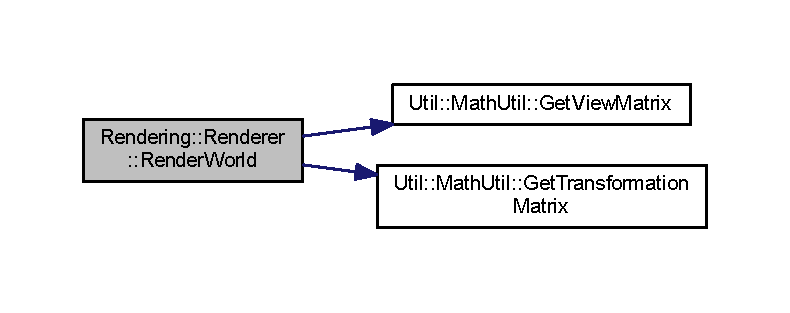
\includegraphics[width=350pt]{class_rendering_1_1_renderer_aeb0226a93b50a1074a7ecacc9e25a88c_cgraph}
\end{center}
\end{figure}
\mbox{\Hypertarget{class_rendering_1_1_renderer_ae5ef00a4de178af3ced56d36327d9c73}\label{class_rendering_1_1_renderer_ae5ef00a4de178af3ced56d36327d9c73}} 
\index{Rendering\+::\+Renderer@{Rendering\+::\+Renderer}!Set\+Dimensions@{Set\+Dimensions}}
\index{Set\+Dimensions@{Set\+Dimensions}!Rendering\+::\+Renderer@{Rendering\+::\+Renderer}}
\subsubsection{\texorpdfstring{Set\+Dimensions()}{SetDimensions()}}
{\footnotesize\ttfamily void Rendering\+::\+Renderer\+::\+Set\+Dimensions (\begin{DoxyParamCaption}\item[{int}]{x,  }\item[{int}]{y }\end{DoxyParamCaption})}

Sets the dimensions of the render target. 
\begin{DoxyParams}[1]{Parameters}
\mbox{\tt in}  & {\em x} & The width of the screen. \\
\hline
\mbox{\tt in}  & {\em y} & The height of the screen. \\
\hline
\end{DoxyParams}


Definition at line 30 of file Renderer.\+cpp.



The documentation for this class was generated from the following files\+:\begin{DoxyCompactItemize}
\item 
Bear\+Bones-\/master/\+Bear\+Bones/src/\+Rendering/Renderer.\+h\item 
Bear\+Bones-\/master/\+Bear\+Bones/src/\+Rendering/Renderer.\+cpp\end{DoxyCompactItemize}

\hypertarget{class_objects_1_1_resource_loader}{}\section{Objects\+:\+:Resource\+Loader Class Reference}
\label{class_objects_1_1_resource_loader}\index{Objects\+::\+Resource\+Loader@{Objects\+::\+Resource\+Loader}}


{\ttfamily \#include $<$Resource\+Loader.\+h$>$}

\subsection*{Public Member Functions}
\begin{DoxyCompactItemize}
\item 
\mbox{\Hypertarget{class_objects_1_1_resource_loader_a7fb135bf2dcf39443bc4daf17909c824}\label{class_objects_1_1_resource_loader_a7fb135bf2dcf39443bc4daf17909c824}} 
{\bfseries Resource\+Loader} (const \hyperlink{class_objects_1_1_resource_loader}{Resource\+Loader} \&other)
\item 
std\+::shared\+\_\+ptr$<$ \hyperlink{class_objects_1_1_texture}{Texture} $>$ \hyperlink{class_objects_1_1_resource_loader_ad1ae22e95d946ef6679f7a21d4cf63d4}{Load\+Texture} (std\+::string filename)
\item 
std\+::shared\+\_\+ptr$<$ \hyperlink{class_objects_1_1_obj_model}{Obj\+Model} $>$ \hyperlink{class_objects_1_1_resource_loader_abc104a8a3963672a9f27419cd64f3930}{Load\+O\+B\+J\+Model} (std\+::string filename, std\+::shared\+\_\+ptr$<$ \hyperlink{class_objects_1_1_texture}{Texture} $>$ texture)
\item 
std\+::shared\+\_\+ptr$<$ \hyperlink{class_objects_1_1_static_entity}{Static\+Entity} $>$ \hyperlink{class_objects_1_1_resource_loader_ac0150dbe31ca7fbbbc2b88127daa36be}{Create\+Static\+Entity} (std\+::shared\+\_\+ptr$<$ \hyperlink{class_objects_1_1_obj_model}{Obj\+Model} $>$ model, glm\+::vec3 position, glm\+::vec3 rotation, glm\+::vec3 scale)
\end{DoxyCompactItemize}


\subsection{Detailed Description}
Contains all the methods required for loading resources into the game. \begin{DoxyAuthor}{Author}
Mathew Causby. 
\end{DoxyAuthor}
\begin{DoxyVersion}{Version}
0.\+1 
\end{DoxyVersion}


Definition at line 29 of file Resource\+Loader.\+h.



\subsection{Member Function Documentation}
\mbox{\Hypertarget{class_objects_1_1_resource_loader_ac0150dbe31ca7fbbbc2b88127daa36be}\label{class_objects_1_1_resource_loader_ac0150dbe31ca7fbbbc2b88127daa36be}} 
\index{Objects\+::\+Resource\+Loader@{Objects\+::\+Resource\+Loader}!Create\+Static\+Entity@{Create\+Static\+Entity}}
\index{Create\+Static\+Entity@{Create\+Static\+Entity}!Objects\+::\+Resource\+Loader@{Objects\+::\+Resource\+Loader}}
\subsubsection{\texorpdfstring{Create\+Static\+Entity()}{CreateStaticEntity()}}
{\footnotesize\ttfamily std\+::shared\+\_\+ptr$<$ \hyperlink{class_objects_1_1_static_entity}{Objects\+::\+Static\+Entity} $>$ Objects\+::\+Resource\+Loader\+::\+Create\+Static\+Entity (\begin{DoxyParamCaption}\item[{std\+::shared\+\_\+ptr$<$ \hyperlink{class_objects_1_1_obj_model}{Obj\+Model} $>$}]{model,  }\item[{glm\+::vec3}]{position,  }\item[{glm\+::vec3}]{rotation,  }\item[{glm\+::vec3}]{scale }\end{DoxyParamCaption})}

Creates a static entity. A static entity is one that won\textquotesingle{}t move or be moved by other objects. 
\begin{DoxyParams}[1]{Parameters}
\mbox{\tt in}  & {\em model} & The model to draw. \\
\hline
\mbox{\tt in}  & {\em position} & The position of the entity. \\
\hline
\mbox{\tt in}  & {\em rotation} & The rotation of the entity. \\
\hline
\mbox{\tt in}  & {\em scale} & The scale of the entity. \\
\hline
\end{DoxyParams}
\begin{DoxySeeAlso}{See also}
\hyperlink{class_objects_1_1_static_entity}{Objects\+::\+Static\+Entity} 
\end{DoxySeeAlso}
\begin{DoxyReturn}{Returns}
A pointer to the newly created entity. 
\end{DoxyReturn}


Definition at line 86 of file Resource\+Loader.\+cpp.

\mbox{\Hypertarget{class_objects_1_1_resource_loader_abc104a8a3963672a9f27419cd64f3930}\label{class_objects_1_1_resource_loader_abc104a8a3963672a9f27419cd64f3930}} 
\index{Objects\+::\+Resource\+Loader@{Objects\+::\+Resource\+Loader}!Load\+O\+B\+J\+Model@{Load\+O\+B\+J\+Model}}
\index{Load\+O\+B\+J\+Model@{Load\+O\+B\+J\+Model}!Objects\+::\+Resource\+Loader@{Objects\+::\+Resource\+Loader}}
\subsubsection{\texorpdfstring{Load\+O\+B\+J\+Model()}{LoadOBJModel()}}
{\footnotesize\ttfamily std\+::shared\+\_\+ptr$<$ \hyperlink{class_objects_1_1_obj_model}{Objects\+::\+Obj\+Model} $>$ Objects\+::\+Resource\+Loader\+::\+Load\+O\+B\+J\+Model (\begin{DoxyParamCaption}\item[{std\+::string}]{filename,  }\item[{std\+::shared\+\_\+ptr$<$ \hyperlink{class_objects_1_1_texture}{Texture} $>$}]{texture }\end{DoxyParamCaption})}

Loads a wavefront object file into the game and uplaods it to a V\+AO and V\+BO\textquotesingle{}s. 
\begin{DoxyParams}[1]{Parameters}
\mbox{\tt in}  & {\em filename} & The filename to load in. \\
\hline
\mbox{\tt in}  & {\em texture} & The texture to assign to the model. \\
\hline
\end{DoxyParams}
\begin{DoxySeeAlso}{See also}
\hyperlink{class_objects_1_1_obj_model}{Objects\+::\+Obj\+Model} 
\end{DoxySeeAlso}
\begin{DoxyReturn}{Returns}
A pointer to the newly created model. 
\end{DoxyReturn}


Definition at line 30 of file Resource\+Loader.\+cpp.

\mbox{\Hypertarget{class_objects_1_1_resource_loader_ad1ae22e95d946ef6679f7a21d4cf63d4}\label{class_objects_1_1_resource_loader_ad1ae22e95d946ef6679f7a21d4cf63d4}} 
\index{Objects\+::\+Resource\+Loader@{Objects\+::\+Resource\+Loader}!Load\+Texture@{Load\+Texture}}
\index{Load\+Texture@{Load\+Texture}!Objects\+::\+Resource\+Loader@{Objects\+::\+Resource\+Loader}}
\subsubsection{\texorpdfstring{Load\+Texture()}{LoadTexture()}}
{\footnotesize\ttfamily std\+::shared\+\_\+ptr$<$ \hyperlink{class_objects_1_1_texture}{Objects\+::\+Texture} $>$ Objects\+::\+Resource\+Loader\+::\+Load\+Texture (\begin{DoxyParamCaption}\item[{std\+::string}]{filename }\end{DoxyParamCaption})}

Loads a texture and uploads to Open\+GL. 
\begin{DoxyParams}[1]{Parameters}
\mbox{\tt in}  & {\em filename} & The filename of the texture. \\
\hline
\end{DoxyParams}
\begin{DoxyReturn}{Returns}
A pointer to the newly created texture file. 
\end{DoxyReturn}
\begin{DoxySeeAlso}{See also}
\hyperlink{class_objects_1_1_texture}{Objects\+::\+Texture} 
\end{DoxySeeAlso}


Definition at line 18 of file Resource\+Loader.\+cpp.



The documentation for this class was generated from the following files\+:\begin{DoxyCompactItemize}
\item 
Bear\+Bones-\/master/\+Bear\+Bones/src/\+Objects/Resource\+Loader.\+h\item 
Bear\+Bones-\/master/\+Bear\+Bones/src/\+Objects/Resource\+Loader.\+cpp\end{DoxyCompactItemize}

\hypertarget{class_shaders_1_1_shader_base}{}\section{Shaders\+:\+:Shader\+Base Class Reference}
\label{class_shaders_1_1_shader_base}\index{Shaders\+::\+Shader\+Base@{Shaders\+::\+Shader\+Base}}


{\ttfamily \#include $<$Shader\+Base.\+h$>$}



Inheritance diagram for Shaders\+:\+:Shader\+Base\+:
\nopagebreak
\begin{figure}[H]
\begin{center}
\leavevmode
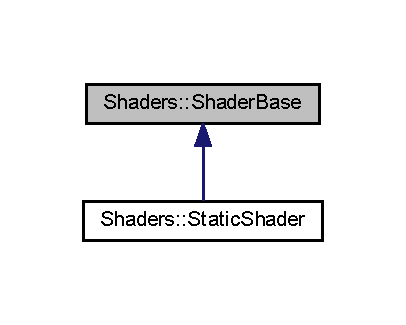
\includegraphics[width=195pt]{class_shaders_1_1_shader_base__inherit__graph}
\end{center}
\end{figure}
\subsection*{Public Member Functions}
\begin{DoxyCompactItemize}
\item 
\mbox{\Hypertarget{class_shaders_1_1_shader_base_a7cc6a08ac2589b24f7667f27b29622df}\label{class_shaders_1_1_shader_base_a7cc6a08ac2589b24f7667f27b29622df}} 
{\bfseries Shader\+Base} (const \hyperlink{class_shaders_1_1_shader_base}{Shader\+Base} \&other)
\item 
void \hyperlink{class_shaders_1_1_shader_base_a70efd0722655ec3dd0c2de014a04fd17}{Start} ()
\item 
void \hyperlink{class_shaders_1_1_shader_base_a1d5f73624ff4f59633b159fd0772e84c}{Stop} ()
\item 
virtual void \hyperlink{class_shaders_1_1_shader_base_a8230f19d72ac58be9db263bbf8436967}{Bind\+Attributes} ()=0
\item 
virtual void \hyperlink{class_shaders_1_1_shader_base_ade949aa1626fbddd264a51b1dbb9a7cc}{Get\+All\+Uniforms} ()=0
\item 
void \hyperlink{class_shaders_1_1_shader_base_a25f6a1f85f7f3094f6019971239ad2ce}{Set\+Program\+ID} (int id)
\item 
void \hyperlink{class_shaders_1_1_shader_base_afb186a683a560e325c3e5fe6f60d6c59}{Set\+Vertex\+Shader\+ID} (int id)
\item 
void \hyperlink{class_shaders_1_1_shader_base_a984b4efce8e3dbb75302017c4f92bb3c}{Set\+Fragment\+Shader\+ID} (int id)
\item 
int \hyperlink{class_shaders_1_1_shader_base_a77870f40caecabf2acbae1eafd38f4c5}{Get\+Program\+ID} ()
\item 
int \hyperlink{class_shaders_1_1_shader_base_afb5d93c464cf2f726557bd4ff43d90ef}{Get\+Vertex\+Shader\+ID} ()
\item 
int \hyperlink{class_shaders_1_1_shader_base_a4cc693649848978b8496359eec993a31}{Get\+Fragment\+Shader\+ID} ()
\end{DoxyCompactItemize}
\subsection*{Protected Member Functions}
\begin{DoxyCompactItemize}
\item 
void \hyperlink{class_shaders_1_1_shader_base_a532cb2422edc5f80c899d702c9f04944}{Bind\+Attrib} (int attrib, const char $\ast$name)
\item 
G\+Luint \hyperlink{class_shaders_1_1_shader_base_ae3fa1c430786dccf85b86e0337fa7f02}{Get\+Uniform} (const char $\ast$name)
\item 
void \hyperlink{class_shaders_1_1_shader_base_ad174cf85ef001561a70461b7e1717129}{Load\+Float} (G\+Luint location, float value)
\item 
void \hyperlink{class_shaders_1_1_shader_base_a039773797967696a8407df9240420464}{Load\+Int} (G\+Luint location, int value)
\item 
void \hyperlink{class_shaders_1_1_shader_base_aaf6da8cee165856e1c34fe04f415fa01}{Load\+U\+Int} (G\+Luint location, unsigned int value)
\item 
void \hyperlink{class_shaders_1_1_shader_base_a2a490771534b22d25458ce05faf275d3}{Load\+Vec3} (G\+Luint location, glm\+::vec3 value)
\item 
void \hyperlink{class_shaders_1_1_shader_base_a0f3ec02c991021e8da69c1ab885624b9}{Load\+Boolean} (G\+Luint location, bool value)
\item 
void \hyperlink{class_shaders_1_1_shader_base_ab6899eacc696db251435d3159851bbd7}{Load\+Matrix4} (G\+Luint location, glm\+::mat4x4 value)
\end{DoxyCompactItemize}


\subsection{Detailed Description}
Abstract class that is the base of all shaders. \begin{DoxyAuthor}{Author}
Mathew Causby 
\end{DoxyAuthor}
\begin{DoxyVersion}{Version}
0.\+1 
\end{DoxyVersion}


Definition at line 18 of file Shader\+Base.\+h.



\subsection{Member Function Documentation}
\mbox{\Hypertarget{class_shaders_1_1_shader_base_a532cb2422edc5f80c899d702c9f04944}\label{class_shaders_1_1_shader_base_a532cb2422edc5f80c899d702c9f04944}} 
\index{Shaders\+::\+Shader\+Base@{Shaders\+::\+Shader\+Base}!Bind\+Attrib@{Bind\+Attrib}}
\index{Bind\+Attrib@{Bind\+Attrib}!Shaders\+::\+Shader\+Base@{Shaders\+::\+Shader\+Base}}
\subsubsection{\texorpdfstring{Bind\+Attrib()}{BindAttrib()}}
{\footnotesize\ttfamily void Shaders\+::\+Shader\+Base\+::\+Bind\+Attrib (\begin{DoxyParamCaption}\item[{int}]{attrib,  }\item[{const char $\ast$}]{name }\end{DoxyParamCaption})\hspace{0.3cm}{\ttfamily [protected]}}

Binds an atribute list to a label/name. 
\begin{DoxyParams}[1]{Parameters}
\mbox{\tt in}  & {\em attrib} & The number of the attribute list. \\
\hline
\mbox{\tt in}  & {\em The} & name to bind it to. \\
\hline
\end{DoxyParams}


Definition at line 58 of file Shader\+Base.\+cpp.

Here is the caller graph for this function\+:
\nopagebreak
\begin{figure}[H]
\begin{center}
\leavevmode
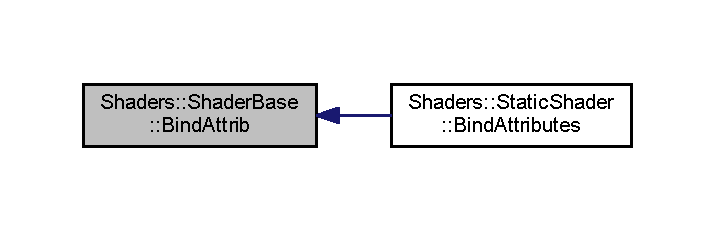
\includegraphics[width=343pt]{class_shaders_1_1_shader_base_a532cb2422edc5f80c899d702c9f04944_icgraph}
\end{center}
\end{figure}
\mbox{\Hypertarget{class_shaders_1_1_shader_base_a8230f19d72ac58be9db263bbf8436967}\label{class_shaders_1_1_shader_base_a8230f19d72ac58be9db263bbf8436967}} 
\index{Shaders\+::\+Shader\+Base@{Shaders\+::\+Shader\+Base}!Bind\+Attributes@{Bind\+Attributes}}
\index{Bind\+Attributes@{Bind\+Attributes}!Shaders\+::\+Shader\+Base@{Shaders\+::\+Shader\+Base}}
\subsubsection{\texorpdfstring{Bind\+Attributes()}{BindAttributes()}}
{\footnotesize\ttfamily virtual void Shaders\+::\+Shader\+Base\+::\+Bind\+Attributes (\begin{DoxyParamCaption}{ }\end{DoxyParamCaption})\hspace{0.3cm}{\ttfamily [pure virtual]}}

Pure virtual function for binding all of the attributes in the shader. 

Implemented in \hyperlink{class_shaders_1_1_static_shader_a4ba0a1e7a4d2b58668f97cb9e3892f57}{Shaders\+::\+Static\+Shader}.

\mbox{\Hypertarget{class_shaders_1_1_shader_base_ade949aa1626fbddd264a51b1dbb9a7cc}\label{class_shaders_1_1_shader_base_ade949aa1626fbddd264a51b1dbb9a7cc}} 
\index{Shaders\+::\+Shader\+Base@{Shaders\+::\+Shader\+Base}!Get\+All\+Uniforms@{Get\+All\+Uniforms}}
\index{Get\+All\+Uniforms@{Get\+All\+Uniforms}!Shaders\+::\+Shader\+Base@{Shaders\+::\+Shader\+Base}}
\subsubsection{\texorpdfstring{Get\+All\+Uniforms()}{GetAllUniforms()}}
{\footnotesize\ttfamily virtual void Shaders\+::\+Shader\+Base\+::\+Get\+All\+Uniforms (\begin{DoxyParamCaption}{ }\end{DoxyParamCaption})\hspace{0.3cm}{\ttfamily [pure virtual]}}

Pure virtual function for getting all of the uniform locations in the shader. 

Implemented in \hyperlink{class_shaders_1_1_static_shader_a2417ca33a617fe8a8cb30ec3b5e866fa}{Shaders\+::\+Static\+Shader}.

\mbox{\Hypertarget{class_shaders_1_1_shader_base_a4cc693649848978b8496359eec993a31}\label{class_shaders_1_1_shader_base_a4cc693649848978b8496359eec993a31}} 
\index{Shaders\+::\+Shader\+Base@{Shaders\+::\+Shader\+Base}!Get\+Fragment\+Shader\+ID@{Get\+Fragment\+Shader\+ID}}
\index{Get\+Fragment\+Shader\+ID@{Get\+Fragment\+Shader\+ID}!Shaders\+::\+Shader\+Base@{Shaders\+::\+Shader\+Base}}
\subsubsection{\texorpdfstring{Get\+Fragment\+Shader\+I\+D()}{GetFragmentShaderID()}}
{\footnotesize\ttfamily int Shaders\+::\+Shader\+Base\+::\+Get\+Fragment\+Shader\+ID (\begin{DoxyParamCaption}{ }\end{DoxyParamCaption})}

Gets the ID of the fragment shader. \begin{DoxyReturn}{Returns}
The ID of the shader. 
\end{DoxyReturn}


Definition at line 53 of file Shader\+Base.\+cpp.

\mbox{\Hypertarget{class_shaders_1_1_shader_base_a77870f40caecabf2acbae1eafd38f4c5}\label{class_shaders_1_1_shader_base_a77870f40caecabf2acbae1eafd38f4c5}} 
\index{Shaders\+::\+Shader\+Base@{Shaders\+::\+Shader\+Base}!Get\+Program\+ID@{Get\+Program\+ID}}
\index{Get\+Program\+ID@{Get\+Program\+ID}!Shaders\+::\+Shader\+Base@{Shaders\+::\+Shader\+Base}}
\subsubsection{\texorpdfstring{Get\+Program\+I\+D()}{GetProgramID()}}
{\footnotesize\ttfamily int Shaders\+::\+Shader\+Base\+::\+Get\+Program\+ID (\begin{DoxyParamCaption}{ }\end{DoxyParamCaption})}

Gets the ID of the entire shader program \begin{DoxyReturn}{Returns}
The ID of the shader. 
\end{DoxyReturn}


Definition at line 43 of file Shader\+Base.\+cpp.

\mbox{\Hypertarget{class_shaders_1_1_shader_base_ae3fa1c430786dccf85b86e0337fa7f02}\label{class_shaders_1_1_shader_base_ae3fa1c430786dccf85b86e0337fa7f02}} 
\index{Shaders\+::\+Shader\+Base@{Shaders\+::\+Shader\+Base}!Get\+Uniform@{Get\+Uniform}}
\index{Get\+Uniform@{Get\+Uniform}!Shaders\+::\+Shader\+Base@{Shaders\+::\+Shader\+Base}}
\subsubsection{\texorpdfstring{Get\+Uniform()}{GetUniform()}}
{\footnotesize\ttfamily G\+Luint Shaders\+::\+Shader\+Base\+::\+Get\+Uniform (\begin{DoxyParamCaption}\item[{const char $\ast$}]{name }\end{DoxyParamCaption})\hspace{0.3cm}{\ttfamily [protected]}}

Gets the location of the uniform with a particular name. 
\begin{DoxyParams}[1]{Parameters}
\mbox{\tt in}  & {\em name} & The name to get the location of. \\
\hline
\end{DoxyParams}
\begin{DoxyReturn}{Returns}
The location of the uniform. 
\end{DoxyReturn}


Definition at line 63 of file Shader\+Base.\+cpp.

Here is the caller graph for this function\+:
\nopagebreak
\begin{figure}[H]
\begin{center}
\leavevmode
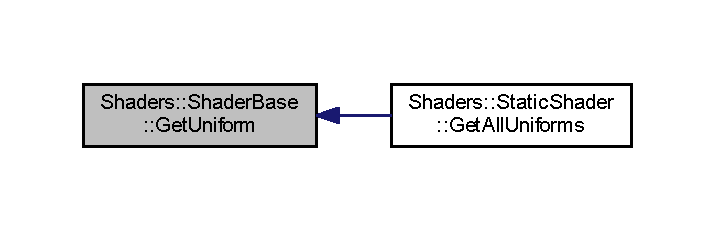
\includegraphics[width=343pt]{class_shaders_1_1_shader_base_ae3fa1c430786dccf85b86e0337fa7f02_icgraph}
\end{center}
\end{figure}
\mbox{\Hypertarget{class_shaders_1_1_shader_base_afb5d93c464cf2f726557bd4ff43d90ef}\label{class_shaders_1_1_shader_base_afb5d93c464cf2f726557bd4ff43d90ef}} 
\index{Shaders\+::\+Shader\+Base@{Shaders\+::\+Shader\+Base}!Get\+Vertex\+Shader\+ID@{Get\+Vertex\+Shader\+ID}}
\index{Get\+Vertex\+Shader\+ID@{Get\+Vertex\+Shader\+ID}!Shaders\+::\+Shader\+Base@{Shaders\+::\+Shader\+Base}}
\subsubsection{\texorpdfstring{Get\+Vertex\+Shader\+I\+D()}{GetVertexShaderID()}}
{\footnotesize\ttfamily int Shaders\+::\+Shader\+Base\+::\+Get\+Vertex\+Shader\+ID (\begin{DoxyParamCaption}{ }\end{DoxyParamCaption})}

Gets the ID of the vertex shader. \begin{DoxyReturn}{Returns}
The ID of the shader. 
\end{DoxyReturn}


Definition at line 48 of file Shader\+Base.\+cpp.

\mbox{\Hypertarget{class_shaders_1_1_shader_base_a0f3ec02c991021e8da69c1ab885624b9}\label{class_shaders_1_1_shader_base_a0f3ec02c991021e8da69c1ab885624b9}} 
\index{Shaders\+::\+Shader\+Base@{Shaders\+::\+Shader\+Base}!Load\+Boolean@{Load\+Boolean}}
\index{Load\+Boolean@{Load\+Boolean}!Shaders\+::\+Shader\+Base@{Shaders\+::\+Shader\+Base}}
\subsubsection{\texorpdfstring{Load\+Boolean()}{LoadBoolean()}}
{\footnotesize\ttfamily void Shaders\+::\+Shader\+Base\+::\+Load\+Boolean (\begin{DoxyParamCaption}\item[{G\+Luint}]{location,  }\item[{bool}]{value }\end{DoxyParamCaption})\hspace{0.3cm}{\ttfamily [protected]}}

Loads a boolean to the shader. 
\begin{DoxyParams}[1]{Parameters}
\mbox{\tt in}  & {\em location} & The location to upload the value to. \\
\hline
\mbox{\tt in}  & {\em value} & The value to upload. \\
\hline
\end{DoxyParams}


Definition at line 88 of file Shader\+Base.\+cpp.

\mbox{\Hypertarget{class_shaders_1_1_shader_base_ad174cf85ef001561a70461b7e1717129}\label{class_shaders_1_1_shader_base_ad174cf85ef001561a70461b7e1717129}} 
\index{Shaders\+::\+Shader\+Base@{Shaders\+::\+Shader\+Base}!Load\+Float@{Load\+Float}}
\index{Load\+Float@{Load\+Float}!Shaders\+::\+Shader\+Base@{Shaders\+::\+Shader\+Base}}
\subsubsection{\texorpdfstring{Load\+Float()}{LoadFloat()}}
{\footnotesize\ttfamily void Shaders\+::\+Shader\+Base\+::\+Load\+Float (\begin{DoxyParamCaption}\item[{G\+Luint}]{location,  }\item[{float}]{value }\end{DoxyParamCaption})\hspace{0.3cm}{\ttfamily [protected]}}

Loads a float to the shader. 
\begin{DoxyParams}[1]{Parameters}
\mbox{\tt in}  & {\em location} & The location to upload the value to. \\
\hline
\mbox{\tt in}  & {\em value} & The value to upload. \\
\hline
\end{DoxyParams}


Definition at line 68 of file Shader\+Base.\+cpp.

\mbox{\Hypertarget{class_shaders_1_1_shader_base_a039773797967696a8407df9240420464}\label{class_shaders_1_1_shader_base_a039773797967696a8407df9240420464}} 
\index{Shaders\+::\+Shader\+Base@{Shaders\+::\+Shader\+Base}!Load\+Int@{Load\+Int}}
\index{Load\+Int@{Load\+Int}!Shaders\+::\+Shader\+Base@{Shaders\+::\+Shader\+Base}}
\subsubsection{\texorpdfstring{Load\+Int()}{LoadInt()}}
{\footnotesize\ttfamily void Shaders\+::\+Shader\+Base\+::\+Load\+Int (\begin{DoxyParamCaption}\item[{G\+Luint}]{location,  }\item[{int}]{value }\end{DoxyParamCaption})\hspace{0.3cm}{\ttfamily [protected]}}

Loads an int to the shader. 
\begin{DoxyParams}[1]{Parameters}
\mbox{\tt in}  & {\em location} & The location to upload the value to. \\
\hline
\mbox{\tt in}  & {\em value} & The value to upload. \\
\hline
\end{DoxyParams}


Definition at line 73 of file Shader\+Base.\+cpp.

\mbox{\Hypertarget{class_shaders_1_1_shader_base_ab6899eacc696db251435d3159851bbd7}\label{class_shaders_1_1_shader_base_ab6899eacc696db251435d3159851bbd7}} 
\index{Shaders\+::\+Shader\+Base@{Shaders\+::\+Shader\+Base}!Load\+Matrix4@{Load\+Matrix4}}
\index{Load\+Matrix4@{Load\+Matrix4}!Shaders\+::\+Shader\+Base@{Shaders\+::\+Shader\+Base}}
\subsubsection{\texorpdfstring{Load\+Matrix4()}{LoadMatrix4()}}
{\footnotesize\ttfamily void Shaders\+::\+Shader\+Base\+::\+Load\+Matrix4 (\begin{DoxyParamCaption}\item[{G\+Luint}]{location,  }\item[{glm\+::mat4x4}]{value }\end{DoxyParamCaption})\hspace{0.3cm}{\ttfamily [protected]}}

Loads a mat4x4 to the shader. 
\begin{DoxyParams}[1]{Parameters}
\mbox{\tt in}  & {\em location} & The location to upload the value to. \\
\hline
\mbox{\tt in}  & {\em value} & The value to upload. \\
\hline
\end{DoxyParams}


Definition at line 93 of file Shader\+Base.\+cpp.

Here is the caller graph for this function\+:
\nopagebreak
\begin{figure}[H]
\begin{center}
\leavevmode
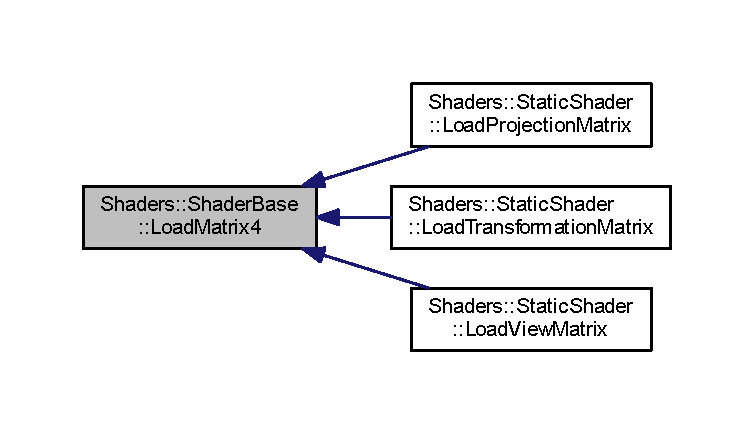
\includegraphics[width=350pt]{class_shaders_1_1_shader_base_ab6899eacc696db251435d3159851bbd7_icgraph}
\end{center}
\end{figure}
\mbox{\Hypertarget{class_shaders_1_1_shader_base_aaf6da8cee165856e1c34fe04f415fa01}\label{class_shaders_1_1_shader_base_aaf6da8cee165856e1c34fe04f415fa01}} 
\index{Shaders\+::\+Shader\+Base@{Shaders\+::\+Shader\+Base}!Load\+U\+Int@{Load\+U\+Int}}
\index{Load\+U\+Int@{Load\+U\+Int}!Shaders\+::\+Shader\+Base@{Shaders\+::\+Shader\+Base}}
\subsubsection{\texorpdfstring{Load\+U\+Int()}{LoadUInt()}}
{\footnotesize\ttfamily void Shaders\+::\+Shader\+Base\+::\+Load\+U\+Int (\begin{DoxyParamCaption}\item[{G\+Luint}]{location,  }\item[{unsigned int}]{value }\end{DoxyParamCaption})\hspace{0.3cm}{\ttfamily [protected]}}

Loads an unsigned int to the shader. 
\begin{DoxyParams}[1]{Parameters}
\mbox{\tt in}  & {\em location} & The location to upload the value to. \\
\hline
\mbox{\tt in}  & {\em value} & The value to upload. \\
\hline
\end{DoxyParams}


Definition at line 78 of file Shader\+Base.\+cpp.

\mbox{\Hypertarget{class_shaders_1_1_shader_base_a2a490771534b22d25458ce05faf275d3}\label{class_shaders_1_1_shader_base_a2a490771534b22d25458ce05faf275d3}} 
\index{Shaders\+::\+Shader\+Base@{Shaders\+::\+Shader\+Base}!Load\+Vec3@{Load\+Vec3}}
\index{Load\+Vec3@{Load\+Vec3}!Shaders\+::\+Shader\+Base@{Shaders\+::\+Shader\+Base}}
\subsubsection{\texorpdfstring{Load\+Vec3()}{LoadVec3()}}
{\footnotesize\ttfamily void Shaders\+::\+Shader\+Base\+::\+Load\+Vec3 (\begin{DoxyParamCaption}\item[{G\+Luint}]{location,  }\item[{glm\+::vec3}]{value }\end{DoxyParamCaption})\hspace{0.3cm}{\ttfamily [protected]}}

Loads a vec3 to the shader. 
\begin{DoxyParams}[1]{Parameters}
\mbox{\tt in}  & {\em location} & The location to upload the value to. \\
\hline
\mbox{\tt in}  & {\em value} & The value to upload. \\
\hline
\end{DoxyParams}


Definition at line 83 of file Shader\+Base.\+cpp.

\mbox{\Hypertarget{class_shaders_1_1_shader_base_a984b4efce8e3dbb75302017c4f92bb3c}\label{class_shaders_1_1_shader_base_a984b4efce8e3dbb75302017c4f92bb3c}} 
\index{Shaders\+::\+Shader\+Base@{Shaders\+::\+Shader\+Base}!Set\+Fragment\+Shader\+ID@{Set\+Fragment\+Shader\+ID}}
\index{Set\+Fragment\+Shader\+ID@{Set\+Fragment\+Shader\+ID}!Shaders\+::\+Shader\+Base@{Shaders\+::\+Shader\+Base}}
\subsubsection{\texorpdfstring{Set\+Fragment\+Shader\+I\+D()}{SetFragmentShaderID()}}
{\footnotesize\ttfamily void Shaders\+::\+Shader\+Base\+::\+Set\+Fragment\+Shader\+ID (\begin{DoxyParamCaption}\item[{int}]{id }\end{DoxyParamCaption})}

Sets the ID of the fragment shader. 
\begin{DoxyParams}[1]{Parameters}
\mbox{\tt in}  & {\em id} & The ID of the shader. \\
\hline
\end{DoxyParams}


Definition at line 38 of file Shader\+Base.\+cpp.

\mbox{\Hypertarget{class_shaders_1_1_shader_base_a25f6a1f85f7f3094f6019971239ad2ce}\label{class_shaders_1_1_shader_base_a25f6a1f85f7f3094f6019971239ad2ce}} 
\index{Shaders\+::\+Shader\+Base@{Shaders\+::\+Shader\+Base}!Set\+Program\+ID@{Set\+Program\+ID}}
\index{Set\+Program\+ID@{Set\+Program\+ID}!Shaders\+::\+Shader\+Base@{Shaders\+::\+Shader\+Base}}
\subsubsection{\texorpdfstring{Set\+Program\+I\+D()}{SetProgramID()}}
{\footnotesize\ttfamily void Shaders\+::\+Shader\+Base\+::\+Set\+Program\+ID (\begin{DoxyParamCaption}\item[{int}]{id }\end{DoxyParamCaption})}

Sets the ID of the entire shader program 
\begin{DoxyParams}[1]{Parameters}
\mbox{\tt in}  & {\em id} & The ID of the shader. \\
\hline
\end{DoxyParams}


Definition at line 28 of file Shader\+Base.\+cpp.

\mbox{\Hypertarget{class_shaders_1_1_shader_base_afb186a683a560e325c3e5fe6f60d6c59}\label{class_shaders_1_1_shader_base_afb186a683a560e325c3e5fe6f60d6c59}} 
\index{Shaders\+::\+Shader\+Base@{Shaders\+::\+Shader\+Base}!Set\+Vertex\+Shader\+ID@{Set\+Vertex\+Shader\+ID}}
\index{Set\+Vertex\+Shader\+ID@{Set\+Vertex\+Shader\+ID}!Shaders\+::\+Shader\+Base@{Shaders\+::\+Shader\+Base}}
\subsubsection{\texorpdfstring{Set\+Vertex\+Shader\+I\+D()}{SetVertexShaderID()}}
{\footnotesize\ttfamily void Shaders\+::\+Shader\+Base\+::\+Set\+Vertex\+Shader\+ID (\begin{DoxyParamCaption}\item[{int}]{id }\end{DoxyParamCaption})}

Sets the ID of the vertex shader. 
\begin{DoxyParams}[1]{Parameters}
\mbox{\tt in}  & {\em id} & The ID of the shader. \\
\hline
\end{DoxyParams}


Definition at line 33 of file Shader\+Base.\+cpp.

\mbox{\Hypertarget{class_shaders_1_1_shader_base_a70efd0722655ec3dd0c2de014a04fd17}\label{class_shaders_1_1_shader_base_a70efd0722655ec3dd0c2de014a04fd17}} 
\index{Shaders\+::\+Shader\+Base@{Shaders\+::\+Shader\+Base}!Start@{Start}}
\index{Start@{Start}!Shaders\+::\+Shader\+Base@{Shaders\+::\+Shader\+Base}}
\subsubsection{\texorpdfstring{Start()}{Start()}}
{\footnotesize\ttfamily void Shaders\+::\+Shader\+Base\+::\+Start (\begin{DoxyParamCaption}{ }\end{DoxyParamCaption})}

Starts the shader. 

Definition at line 18 of file Shader\+Base.\+cpp.

\mbox{\Hypertarget{class_shaders_1_1_shader_base_a1d5f73624ff4f59633b159fd0772e84c}\label{class_shaders_1_1_shader_base_a1d5f73624ff4f59633b159fd0772e84c}} 
\index{Shaders\+::\+Shader\+Base@{Shaders\+::\+Shader\+Base}!Stop@{Stop}}
\index{Stop@{Stop}!Shaders\+::\+Shader\+Base@{Shaders\+::\+Shader\+Base}}
\subsubsection{\texorpdfstring{Stop()}{Stop()}}
{\footnotesize\ttfamily void Shaders\+::\+Shader\+Base\+::\+Stop (\begin{DoxyParamCaption}{ }\end{DoxyParamCaption})}

Stops the shader. 

Definition at line 23 of file Shader\+Base.\+cpp.



The documentation for this class was generated from the following files\+:\begin{DoxyCompactItemize}
\item 
Bear\+Bones-\/master/\+Bear\+Bones/src/\+Shaders/Shader\+Base.\+h\item 
Bear\+Bones-\/master/\+Bear\+Bones/src/\+Shaders/Shader\+Base.\+cpp\end{DoxyCompactItemize}

\hypertarget{class_objects_1_1_static_entity}{}\section{Objects\+:\+:Static\+Entity Class Reference}
\label{class_objects_1_1_static_entity}\index{Objects\+::\+Static\+Entity@{Objects\+::\+Static\+Entity}}


{\ttfamily \#include $<$Static\+Entity.\+h$>$}



Inheritance diagram for Objects\+:\+:Static\+Entity\+:
\nopagebreak
\begin{figure}[H]
\begin{center}
\leavevmode
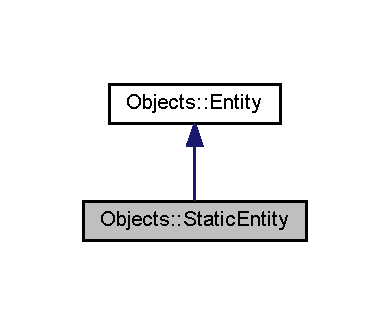
\includegraphics[width=187pt]{class_objects_1_1_static_entity__inherit__graph}
\end{center}
\end{figure}


Collaboration diagram for Objects\+:\+:Static\+Entity\+:
\nopagebreak
\begin{figure}[H]
\begin{center}
\leavevmode
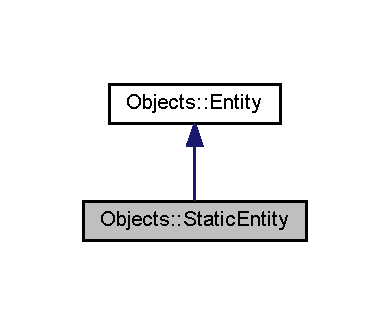
\includegraphics[width=187pt]{class_objects_1_1_static_entity__coll__graph}
\end{center}
\end{figure}
\subsection*{Public Member Functions}
\begin{DoxyCompactItemize}
\item 
\mbox{\Hypertarget{class_objects_1_1_static_entity_ae611b292618ebfc8fff200dbbf8080e6}\label{class_objects_1_1_static_entity_ae611b292618ebfc8fff200dbbf8080e6}} 
{\bfseries Static\+Entity} (const \hyperlink{class_objects_1_1_static_entity}{Static\+Entity} \&other)
\item 
\mbox{\Hypertarget{class_objects_1_1_static_entity_a173c0997cfd7cfb323230a98a9884775}\label{class_objects_1_1_static_entity_a173c0997cfd7cfb323230a98a9884775}} 
{\bfseries Static\+Entity} (const \hyperlink{class_objects_1_1_entity}{Entity} \&other)
\item 
void \hyperlink{class_objects_1_1_static_entity_ae4b1ecdb50494a6d784b81803041ed52}{Create\+Bounding\+Box} ()
\end{DoxyCompactItemize}


\subsection{Detailed Description}
A static entity is an entity that won\textquotesingle{}t move or be moved by other entities. \begin{DoxyAuthor}{Author}
Mathew Causby 
\end{DoxyAuthor}
\begin{DoxyVersion}{Version}
0.\+1 
\end{DoxyVersion}


Definition at line 14 of file Static\+Entity.\+h.



\subsection{Member Function Documentation}
\mbox{\Hypertarget{class_objects_1_1_static_entity_ae4b1ecdb50494a6d784b81803041ed52}\label{class_objects_1_1_static_entity_ae4b1ecdb50494a6d784b81803041ed52}} 
\index{Objects\+::\+Static\+Entity@{Objects\+::\+Static\+Entity}!Create\+Bounding\+Box@{Create\+Bounding\+Box}}
\index{Create\+Bounding\+Box@{Create\+Bounding\+Box}!Objects\+::\+Static\+Entity@{Objects\+::\+Static\+Entity}}
\subsubsection{\texorpdfstring{Create\+Bounding\+Box()}{CreateBoundingBox()}}
{\footnotesize\ttfamily void Objects\+::\+Static\+Entity\+::\+Create\+Bounding\+Box (\begin{DoxyParamCaption}{ }\end{DoxyParamCaption})\hspace{0.3cm}{\ttfamily [virtual]}}

Creates a bounding box for the \hyperlink{class_objects_1_1_static_entity}{Static\+Entity}. Static entities use A\+A\+BB. 

Implements \hyperlink{class_objects_1_1_entity_a3fc51fcad3f731410589f7ab0e3dbe7e}{Objects\+::\+Entity}.



Definition at line 23 of file Static\+Entity.\+cpp.



The documentation for this class was generated from the following files\+:\begin{DoxyCompactItemize}
\item 
Bear\+Bones-\/master/\+Bear\+Bones/src/\+Objects/Static\+Entity.\+h\item 
Bear\+Bones-\/master/\+Bear\+Bones/src/\+Objects/Static\+Entity.\+cpp\end{DoxyCompactItemize}

\hypertarget{class_shaders_1_1_static_shader}{}\section{Shaders\+:\+:Static\+Shader Class Reference}
\label{class_shaders_1_1_static_shader}\index{Shaders\+::\+Static\+Shader@{Shaders\+::\+Static\+Shader}}


{\ttfamily \#include $<$Static\+Shader.\+h$>$}



Inheritance diagram for Shaders\+:\+:Static\+Shader\+:
\nopagebreak
\begin{figure}[H]
\begin{center}
\leavevmode
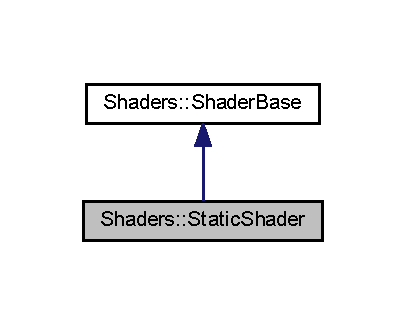
\includegraphics[width=195pt]{class_shaders_1_1_static_shader__inherit__graph}
\end{center}
\end{figure}


Collaboration diagram for Shaders\+:\+:Static\+Shader\+:
\nopagebreak
\begin{figure}[H]
\begin{center}
\leavevmode
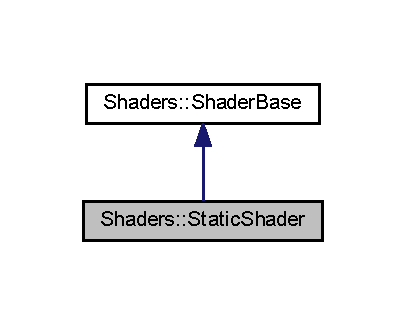
\includegraphics[width=195pt]{class_shaders_1_1_static_shader__coll__graph}
\end{center}
\end{figure}
\subsection*{Public Member Functions}
\begin{DoxyCompactItemize}
\item 
\mbox{\Hypertarget{class_shaders_1_1_static_shader_a133b2935aef11a9e51bf2589a1400f4b}\label{class_shaders_1_1_static_shader_a133b2935aef11a9e51bf2589a1400f4b}} 
{\bfseries Static\+Shader} (const \hyperlink{class_shaders_1_1_static_shader}{Static\+Shader} \&other)
\item 
void \hyperlink{class_shaders_1_1_static_shader_a4ba0a1e7a4d2b58668f97cb9e3892f57}{Bind\+Attributes} ()
\item 
void \hyperlink{class_shaders_1_1_static_shader_a2417ca33a617fe8a8cb30ec3b5e866fa}{Get\+All\+Uniforms} ()
\item 
void \hyperlink{class_shaders_1_1_static_shader_a7133b5436145e2769cb940835e59a5f7}{Load\+Projection\+Matrix} (glm\+::mat4x4 projection\+Matrix)
\item 
void \hyperlink{class_shaders_1_1_static_shader_ab0241a6caf6b7a9fe48b35da63a1cefb}{Load\+Transformation\+Matrix} (glm\+::mat4x4 transformation\+Matrix)
\item 
void \hyperlink{class_shaders_1_1_static_shader_aacb252f60950b03d3aa0dc0abc92d768}{Load\+View\+Matrix} (glm\+::mat4x4 view\+Matrix)
\end{DoxyCompactItemize}
\subsection*{Additional Inherited Members}


\subsection{Detailed Description}
Implementation of \hyperlink{class_shaders_1_1_shader_base}{Shader\+Base} defining a shader for static objects. That is objects without animation. Also uploads the projection, transformation, and view matricies to the shader to create the M\+VP transformation. \begin{DoxyAuthor}{Author}
Mathew Causby 
\end{DoxyAuthor}
\begin{DoxyVersion}{Version}
0.\+1 
\end{DoxyVersion}


Definition at line 15 of file Static\+Shader.\+h.



\subsection{Member Function Documentation}
\mbox{\Hypertarget{class_shaders_1_1_static_shader_a4ba0a1e7a4d2b58668f97cb9e3892f57}\label{class_shaders_1_1_static_shader_a4ba0a1e7a4d2b58668f97cb9e3892f57}} 
\index{Shaders\+::\+Static\+Shader@{Shaders\+::\+Static\+Shader}!Bind\+Attributes@{Bind\+Attributes}}
\index{Bind\+Attributes@{Bind\+Attributes}!Shaders\+::\+Static\+Shader@{Shaders\+::\+Static\+Shader}}
\subsubsection{\texorpdfstring{Bind\+Attributes()}{BindAttributes()}}
{\footnotesize\ttfamily void Shaders\+::\+Static\+Shader\+::\+Bind\+Attributes (\begin{DoxyParamCaption}{ }\end{DoxyParamCaption})\hspace{0.3cm}{\ttfamily [virtual]}}

Binds all the attributes to the shader. 

Implements \hyperlink{class_shaders_1_1_shader_base_a8230f19d72ac58be9db263bbf8436967}{Shaders\+::\+Shader\+Base}.



Definition at line 18 of file Static\+Shader.\+cpp.

Here is the call graph for this function\+:
\nopagebreak
\begin{figure}[H]
\begin{center}
\leavevmode
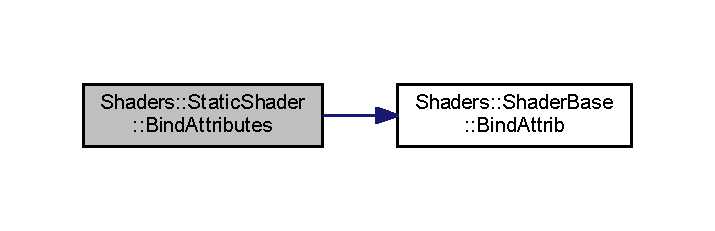
\includegraphics[width=343pt]{class_shaders_1_1_static_shader_a4ba0a1e7a4d2b58668f97cb9e3892f57_cgraph}
\end{center}
\end{figure}
\mbox{\Hypertarget{class_shaders_1_1_static_shader_a2417ca33a617fe8a8cb30ec3b5e866fa}\label{class_shaders_1_1_static_shader_a2417ca33a617fe8a8cb30ec3b5e866fa}} 
\index{Shaders\+::\+Static\+Shader@{Shaders\+::\+Static\+Shader}!Get\+All\+Uniforms@{Get\+All\+Uniforms}}
\index{Get\+All\+Uniforms@{Get\+All\+Uniforms}!Shaders\+::\+Static\+Shader@{Shaders\+::\+Static\+Shader}}
\subsubsection{\texorpdfstring{Get\+All\+Uniforms()}{GetAllUniforms()}}
{\footnotesize\ttfamily void Shaders\+::\+Static\+Shader\+::\+Get\+All\+Uniforms (\begin{DoxyParamCaption}{ }\end{DoxyParamCaption})\hspace{0.3cm}{\ttfamily [virtual]}}

Gets the location of all the unfiforms in the shader. 

Implements \hyperlink{class_shaders_1_1_shader_base_ade949aa1626fbddd264a51b1dbb9a7cc}{Shaders\+::\+Shader\+Base}.



Definition at line 25 of file Static\+Shader.\+cpp.

Here is the call graph for this function\+:
\nopagebreak
\begin{figure}[H]
\begin{center}
\leavevmode
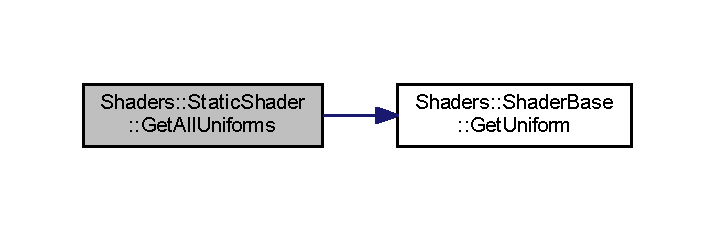
\includegraphics[width=343pt]{class_shaders_1_1_static_shader_a2417ca33a617fe8a8cb30ec3b5e866fa_cgraph}
\end{center}
\end{figure}
\mbox{\Hypertarget{class_shaders_1_1_static_shader_a7133b5436145e2769cb940835e59a5f7}\label{class_shaders_1_1_static_shader_a7133b5436145e2769cb940835e59a5f7}} 
\index{Shaders\+::\+Static\+Shader@{Shaders\+::\+Static\+Shader}!Load\+Projection\+Matrix@{Load\+Projection\+Matrix}}
\index{Load\+Projection\+Matrix@{Load\+Projection\+Matrix}!Shaders\+::\+Static\+Shader@{Shaders\+::\+Static\+Shader}}
\subsubsection{\texorpdfstring{Load\+Projection\+Matrix()}{LoadProjectionMatrix()}}
{\footnotesize\ttfamily void Shaders\+::\+Static\+Shader\+::\+Load\+Projection\+Matrix (\begin{DoxyParamCaption}\item[{glm\+::mat4x4}]{projection\+Matrix }\end{DoxyParamCaption})}

Loads the projection matrix to the shader. 
\begin{DoxyParams}[1]{Parameters}
\mbox{\tt in}  & {\em projection\+Matrix} & The projection matrix. \\
\hline
\end{DoxyParams}


Definition at line 32 of file Static\+Shader.\+cpp.

Here is the call graph for this function\+:
\nopagebreak
\begin{figure}[H]
\begin{center}
\leavevmode
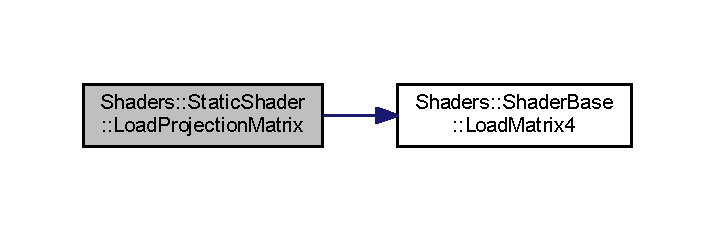
\includegraphics[width=343pt]{class_shaders_1_1_static_shader_a7133b5436145e2769cb940835e59a5f7_cgraph}
\end{center}
\end{figure}
\mbox{\Hypertarget{class_shaders_1_1_static_shader_ab0241a6caf6b7a9fe48b35da63a1cefb}\label{class_shaders_1_1_static_shader_ab0241a6caf6b7a9fe48b35da63a1cefb}} 
\index{Shaders\+::\+Static\+Shader@{Shaders\+::\+Static\+Shader}!Load\+Transformation\+Matrix@{Load\+Transformation\+Matrix}}
\index{Load\+Transformation\+Matrix@{Load\+Transformation\+Matrix}!Shaders\+::\+Static\+Shader@{Shaders\+::\+Static\+Shader}}
\subsubsection{\texorpdfstring{Load\+Transformation\+Matrix()}{LoadTransformationMatrix()}}
{\footnotesize\ttfamily void Shaders\+::\+Static\+Shader\+::\+Load\+Transformation\+Matrix (\begin{DoxyParamCaption}\item[{glm\+::mat4x4}]{transformation\+Matrix }\end{DoxyParamCaption})}

Loads the transformation matrix to the shader. 
\begin{DoxyParams}[1]{Parameters}
\mbox{\tt in}  & {\em transformation\+Matrix} & The transformation matrix. \\
\hline
\end{DoxyParams}


Definition at line 37 of file Static\+Shader.\+cpp.

Here is the call graph for this function\+:
\nopagebreak
\begin{figure}[H]
\begin{center}
\leavevmode
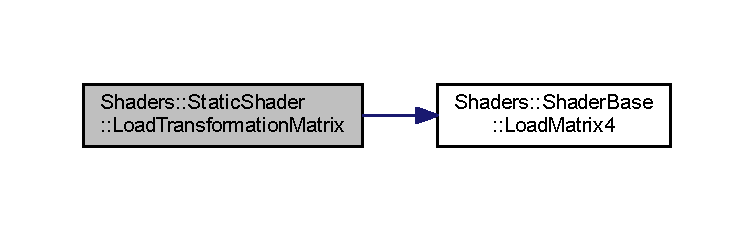
\includegraphics[width=350pt]{class_shaders_1_1_static_shader_ab0241a6caf6b7a9fe48b35da63a1cefb_cgraph}
\end{center}
\end{figure}
\mbox{\Hypertarget{class_shaders_1_1_static_shader_aacb252f60950b03d3aa0dc0abc92d768}\label{class_shaders_1_1_static_shader_aacb252f60950b03d3aa0dc0abc92d768}} 
\index{Shaders\+::\+Static\+Shader@{Shaders\+::\+Static\+Shader}!Load\+View\+Matrix@{Load\+View\+Matrix}}
\index{Load\+View\+Matrix@{Load\+View\+Matrix}!Shaders\+::\+Static\+Shader@{Shaders\+::\+Static\+Shader}}
\subsubsection{\texorpdfstring{Load\+View\+Matrix()}{LoadViewMatrix()}}
{\footnotesize\ttfamily void Shaders\+::\+Static\+Shader\+::\+Load\+View\+Matrix (\begin{DoxyParamCaption}\item[{glm\+::mat4x4}]{view\+Matrix }\end{DoxyParamCaption})}

Loads the view matrix to the shader. 
\begin{DoxyParams}[1]{Parameters}
\mbox{\tt in}  & {\em view\+Matrix} & The view matrix. \\
\hline
\end{DoxyParams}


Definition at line 42 of file Static\+Shader.\+cpp.

Here is the call graph for this function\+:
\nopagebreak
\begin{figure}[H]
\begin{center}
\leavevmode
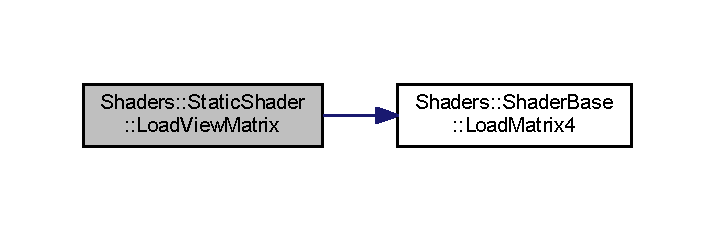
\includegraphics[width=343pt]{class_shaders_1_1_static_shader_aacb252f60950b03d3aa0dc0abc92d768_cgraph}
\end{center}
\end{figure}


The documentation for this class was generated from the following files\+:\begin{DoxyCompactItemize}
\item 
Bear\+Bones-\/master/\+Bear\+Bones/src/\+Shaders/Static\+Shader.\+h\item 
Bear\+Bones-\/master/\+Bear\+Bones/src/\+Shaders/Static\+Shader.\+cpp\end{DoxyCompactItemize}

\hypertarget{class_objects_1_1_texture}{}\section{Objects\+:\+:Texture Class Reference}
\label{class_objects_1_1_texture}\index{Objects\+::\+Texture@{Objects\+::\+Texture}}


{\ttfamily \#include $<$Texture.\+h$>$}

\subsection*{Public Member Functions}
\begin{DoxyCompactItemize}
\item 
\mbox{\Hypertarget{class_objects_1_1_texture_a8227f3e1a2240abafaeec2a911adfbff}\label{class_objects_1_1_texture_a8227f3e1a2240abafaeec2a911adfbff}} 
{\bfseries Texture} (const \hyperlink{class_objects_1_1_texture}{Texture} \&other)
\item 
void \hyperlink{class_objects_1_1_texture_a1964a04cbe93f6040f19238f51c98616}{Bind} ()
\item 
void \hyperlink{class_objects_1_1_texture_aecfe36e814417cf874c1145f28320f7f}{Unbind} ()
\item 
void \hyperlink{class_objects_1_1_texture_a50e08a5bbec2568ac45ba2d49d3c1dbd}{Destroy} ()
\item 
void \hyperlink{class_objects_1_1_texture_ab64d6c23647133c9bd86ca9a457bae77}{Set\+Texture\+ID} (int tex\+Id)
\item 
int \hyperlink{class_objects_1_1_texture_a6d1a2e5398eab5d19ef717638305f9c4}{Get\+Texture\+ID} ()
\end{DoxyCompactItemize}


\subsection{Detailed Description}
A texture defines the information about the texture, as well as helper methods to bind and unbind the texture. \begin{DoxyAuthor}{Author}
Mathew Causby 
\end{DoxyAuthor}
\begin{DoxyVersion}{Version}
0.\+1 
\end{DoxyVersion}


Definition at line 13 of file Texture.\+h.



\subsection{Member Function Documentation}
\mbox{\Hypertarget{class_objects_1_1_texture_a1964a04cbe93f6040f19238f51c98616}\label{class_objects_1_1_texture_a1964a04cbe93f6040f19238f51c98616}} 
\index{Objects\+::\+Texture@{Objects\+::\+Texture}!Bind@{Bind}}
\index{Bind@{Bind}!Objects\+::\+Texture@{Objects\+::\+Texture}}
\subsubsection{\texorpdfstring{Bind()}{Bind()}}
{\footnotesize\ttfamily void Objects\+::\+Texture\+::\+Bind (\begin{DoxyParamCaption}{ }\end{DoxyParamCaption})}

Binds the texture so that it can be drawn over a model. 

Definition at line 18 of file Texture.\+cpp.

\mbox{\Hypertarget{class_objects_1_1_texture_a50e08a5bbec2568ac45ba2d49d3c1dbd}\label{class_objects_1_1_texture_a50e08a5bbec2568ac45ba2d49d3c1dbd}} 
\index{Objects\+::\+Texture@{Objects\+::\+Texture}!Destroy@{Destroy}}
\index{Destroy@{Destroy}!Objects\+::\+Texture@{Objects\+::\+Texture}}
\subsubsection{\texorpdfstring{Destroy()}{Destroy()}}
{\footnotesize\ttfamily void Objects\+::\+Texture\+::\+Destroy (\begin{DoxyParamCaption}{ }\end{DoxyParamCaption})}

Destroys the texture and free\textquotesingle{}s the memory. 

Definition at line 28 of file Texture.\+cpp.

\mbox{\Hypertarget{class_objects_1_1_texture_a6d1a2e5398eab5d19ef717638305f9c4}\label{class_objects_1_1_texture_a6d1a2e5398eab5d19ef717638305f9c4}} 
\index{Objects\+::\+Texture@{Objects\+::\+Texture}!Get\+Texture\+ID@{Get\+Texture\+ID}}
\index{Get\+Texture\+ID@{Get\+Texture\+ID}!Objects\+::\+Texture@{Objects\+::\+Texture}}
\subsubsection{\texorpdfstring{Get\+Texture\+I\+D()}{GetTextureID()}}
{\footnotesize\ttfamily int Objects\+::\+Texture\+::\+Get\+Texture\+ID (\begin{DoxyParamCaption}{ }\end{DoxyParamCaption})}

Gets the texture ID. \begin{DoxyReturn}{Returns}
The ID of the texture. 
\end{DoxyReturn}


Definition at line 38 of file Texture.\+cpp.

\mbox{\Hypertarget{class_objects_1_1_texture_ab64d6c23647133c9bd86ca9a457bae77}\label{class_objects_1_1_texture_ab64d6c23647133c9bd86ca9a457bae77}} 
\index{Objects\+::\+Texture@{Objects\+::\+Texture}!Set\+Texture\+ID@{Set\+Texture\+ID}}
\index{Set\+Texture\+ID@{Set\+Texture\+ID}!Objects\+::\+Texture@{Objects\+::\+Texture}}
\subsubsection{\texorpdfstring{Set\+Texture\+I\+D()}{SetTextureID()}}
{\footnotesize\ttfamily void Objects\+::\+Texture\+::\+Set\+Texture\+ID (\begin{DoxyParamCaption}\item[{int}]{tex\+Id }\end{DoxyParamCaption})}

Sets the texture ID generated by Open\+GL. 
\begin{DoxyParams}[1]{Parameters}
\mbox{\tt in}  & {\em tex\+Id} & The ID of the texture. \\
\hline
\end{DoxyParams}


Definition at line 33 of file Texture.\+cpp.

\mbox{\Hypertarget{class_objects_1_1_texture_aecfe36e814417cf874c1145f28320f7f}\label{class_objects_1_1_texture_aecfe36e814417cf874c1145f28320f7f}} 
\index{Objects\+::\+Texture@{Objects\+::\+Texture}!Unbind@{Unbind}}
\index{Unbind@{Unbind}!Objects\+::\+Texture@{Objects\+::\+Texture}}
\subsubsection{\texorpdfstring{Unbind()}{Unbind()}}
{\footnotesize\ttfamily void Objects\+::\+Texture\+::\+Unbind (\begin{DoxyParamCaption}{ }\end{DoxyParamCaption})}

Unbinds the texture. 

Definition at line 23 of file Texture.\+cpp.



The documentation for this class was generated from the following files\+:\begin{DoxyCompactItemize}
\item 
Bear\+Bones-\/master/\+Bear\+Bones/src/\+Objects/Texture.\+h\item 
Bear\+Bones-\/master/\+Bear\+Bones/src/\+Objects/Texture.\+cpp\end{DoxyCompactItemize}

\hypertarget{class_objects_1_1_world}{}\section{Objects\+:\+:World Class Reference}
\label{class_objects_1_1_world}\index{Objects\+::\+World@{Objects\+::\+World}}


{\ttfamily \#include $<$World.\+h$>$}

\subsection*{Public Member Functions}
\begin{DoxyCompactItemize}
\item 
\mbox{\Hypertarget{class_objects_1_1_world_ae94afd14baa2b242fe12612a6a0a229b}\label{class_objects_1_1_world_ae94afd14baa2b242fe12612a6a0a229b}} 
{\bfseries World} (const \hyperlink{class_objects_1_1_world}{World} \&other)
\item 
void \hyperlink{class_objects_1_1_world_af564fbdf334909ccc2e625be04d05b65}{Add\+Texture} (std\+::shared\+\_\+ptr$<$ \hyperlink{class_objects_1_1_texture}{Texture} $>$ texture)
\item 
void \hyperlink{class_objects_1_1_world_ad84eb295fb787e7217237e27560f1e41}{Add\+Obj\+Model} (std\+::shared\+\_\+ptr$<$ \hyperlink{class_objects_1_1_obj_model}{Obj\+Model} $>$ model)
\item 
void \hyperlink{class_objects_1_1_world_a8512010f2e623aafdeb68b86fc8a5efa}{Add\+Static\+Entity} (std\+::shared\+\_\+ptr$<$ \hyperlink{class_objects_1_1_static_entity}{Static\+Entity} $>$ entity)
\item 
std\+::shared\+\_\+ptr$<$ std\+::vector$<$ std\+::shared\+\_\+ptr$<$ \hyperlink{class_objects_1_1_texture}{Texture} $>$ $>$ $>$ \hyperlink{class_objects_1_1_world_a64f1de04ba2b729474135a8af6ac3163}{Get\+Textures} ()
\item 
std\+::shared\+\_\+ptr$<$ std\+::vector$<$ std\+::shared\+\_\+ptr$<$ \hyperlink{class_objects_1_1_obj_model}{Obj\+Model} $>$ $>$ $>$ \hyperlink{class_objects_1_1_world_a09762556086e4534f26af0e6092d794a}{Get\+O\+B\+J\+Models} ()
\item 
std\+::shared\+\_\+ptr$<$ std\+::vector$<$ std\+::shared\+\_\+ptr$<$ \hyperlink{class_objects_1_1_static_entity}{Static\+Entity} $>$ $>$ $>$ \hyperlink{class_objects_1_1_world_a8f430397fa8f3c30d2105f8d7e5268e3}{Get\+Static\+Entities} ()
\end{DoxyCompactItemize}


\subsection{Detailed Description}
The world object contains all the resources used in the game. \begin{DoxyAuthor}{Author}
Mathew Causby. 
\end{DoxyAuthor}
\begin{DoxyVersion}{Version}
0.\+1 
\end{DoxyVersion}


Definition at line 19 of file World.\+h.



\subsection{Member Function Documentation}
\mbox{\Hypertarget{class_objects_1_1_world_ad84eb295fb787e7217237e27560f1e41}\label{class_objects_1_1_world_ad84eb295fb787e7217237e27560f1e41}} 
\index{Objects\+::\+World@{Objects\+::\+World}!Add\+Obj\+Model@{Add\+Obj\+Model}}
\index{Add\+Obj\+Model@{Add\+Obj\+Model}!Objects\+::\+World@{Objects\+::\+World}}
\subsubsection{\texorpdfstring{Add\+Obj\+Model()}{AddObjModel()}}
{\footnotesize\ttfamily void Objects\+::\+World\+::\+Add\+Obj\+Model (\begin{DoxyParamCaption}\item[{std\+::shared\+\_\+ptr$<$ \hyperlink{class_objects_1_1_obj_model}{Obj\+Model} $>$}]{model }\end{DoxyParamCaption})}

Adds an \hyperlink{class_objects_1_1_obj_model}{Obj\+Model} to the world 
\begin{DoxyParams}[1]{Parameters}
\mbox{\tt in}  & {\em A} & pointer to the \hyperlink{class_objects_1_1_obj_model}{Obj\+Model} \\
\hline
\end{DoxyParams}
\begin{DoxySeeAlso}{See also}
\hyperlink{class_objects_1_1_obj_model}{Objects\+::\+Obj\+Model} 
\end{DoxySeeAlso}


Definition at line 27 of file World.\+cpp.

\mbox{\Hypertarget{class_objects_1_1_world_a8512010f2e623aafdeb68b86fc8a5efa}\label{class_objects_1_1_world_a8512010f2e623aafdeb68b86fc8a5efa}} 
\index{Objects\+::\+World@{Objects\+::\+World}!Add\+Static\+Entity@{Add\+Static\+Entity}}
\index{Add\+Static\+Entity@{Add\+Static\+Entity}!Objects\+::\+World@{Objects\+::\+World}}
\subsubsection{\texorpdfstring{Add\+Static\+Entity()}{AddStaticEntity()}}
{\footnotesize\ttfamily void Objects\+::\+World\+::\+Add\+Static\+Entity (\begin{DoxyParamCaption}\item[{std\+::shared\+\_\+ptr$<$ \hyperlink{class_objects_1_1_static_entity}{Static\+Entity} $>$}]{entity }\end{DoxyParamCaption})}

Adds a static entity to the world 
\begin{DoxyParams}[1]{Parameters}
\mbox{\tt in}  & {\em A} & pointer to the static entity. \\
\hline
\end{DoxyParams}
\begin{DoxySeeAlso}{See also}
\hyperlink{class_objects_1_1_static_entity}{Objects\+::\+Static\+Entity} 
\end{DoxySeeAlso}


Definition at line 32 of file World.\+cpp.

\mbox{\Hypertarget{class_objects_1_1_world_af564fbdf334909ccc2e625be04d05b65}\label{class_objects_1_1_world_af564fbdf334909ccc2e625be04d05b65}} 
\index{Objects\+::\+World@{Objects\+::\+World}!Add\+Texture@{Add\+Texture}}
\index{Add\+Texture@{Add\+Texture}!Objects\+::\+World@{Objects\+::\+World}}
\subsubsection{\texorpdfstring{Add\+Texture()}{AddTexture()}}
{\footnotesize\ttfamily void Objects\+::\+World\+::\+Add\+Texture (\begin{DoxyParamCaption}\item[{std\+::shared\+\_\+ptr$<$ \hyperlink{class_objects_1_1_texture}{Texture} $>$}]{texture }\end{DoxyParamCaption})}

Adds a texture to the world. 
\begin{DoxyParams}[1]{Parameters}
\mbox{\tt in}  & {\em A} & pointer to the texture. \\
\hline
\end{DoxyParams}
\begin{DoxySeeAlso}{See also}
\hyperlink{class_objects_1_1_texture}{Objects\+::\+Texture} 
\end{DoxySeeAlso}


Definition at line 22 of file World.\+cpp.

\mbox{\Hypertarget{class_objects_1_1_world_a09762556086e4534f26af0e6092d794a}\label{class_objects_1_1_world_a09762556086e4534f26af0e6092d794a}} 
\index{Objects\+::\+World@{Objects\+::\+World}!Get\+O\+B\+J\+Models@{Get\+O\+B\+J\+Models}}
\index{Get\+O\+B\+J\+Models@{Get\+O\+B\+J\+Models}!Objects\+::\+World@{Objects\+::\+World}}
\subsubsection{\texorpdfstring{Get\+O\+B\+J\+Models()}{GetOBJModels()}}
{\footnotesize\ttfamily std\+::shared\+\_\+ptr$<$ std\+::vector$<$ std\+::shared\+\_\+ptr$<$ \hyperlink{class_objects_1_1_obj_model}{Objects\+::\+Obj\+Model} $>$ $>$ $>$ Objects\+::\+World\+::\+Get\+O\+B\+J\+Models (\begin{DoxyParamCaption}{ }\end{DoxyParamCaption})}

Gets the obj models currently loaded. \begin{DoxyReturn}{Returns}
A vector of pointers to models currently in the world. 
\end{DoxyReturn}


Definition at line 42 of file World.\+cpp.

\mbox{\Hypertarget{class_objects_1_1_world_a8f430397fa8f3c30d2105f8d7e5268e3}\label{class_objects_1_1_world_a8f430397fa8f3c30d2105f8d7e5268e3}} 
\index{Objects\+::\+World@{Objects\+::\+World}!Get\+Static\+Entities@{Get\+Static\+Entities}}
\index{Get\+Static\+Entities@{Get\+Static\+Entities}!Objects\+::\+World@{Objects\+::\+World}}
\subsubsection{\texorpdfstring{Get\+Static\+Entities()}{GetStaticEntities()}}
{\footnotesize\ttfamily std\+::shared\+\_\+ptr$<$ std\+::vector$<$ std\+::shared\+\_\+ptr$<$ \hyperlink{class_objects_1_1_static_entity}{Objects\+::\+Static\+Entity} $>$ $>$ $>$ Objects\+::\+World\+::\+Get\+Static\+Entities (\begin{DoxyParamCaption}{ }\end{DoxyParamCaption})}

Gets the static entities currently loaded. \begin{DoxyReturn}{Returns}
A vector of pointers to static entities currently in the world. 
\end{DoxyReturn}


Definition at line 47 of file World.\+cpp.

\mbox{\Hypertarget{class_objects_1_1_world_a64f1de04ba2b729474135a8af6ac3163}\label{class_objects_1_1_world_a64f1de04ba2b729474135a8af6ac3163}} 
\index{Objects\+::\+World@{Objects\+::\+World}!Get\+Textures@{Get\+Textures}}
\index{Get\+Textures@{Get\+Textures}!Objects\+::\+World@{Objects\+::\+World}}
\subsubsection{\texorpdfstring{Get\+Textures()}{GetTextures()}}
{\footnotesize\ttfamily std\+::shared\+\_\+ptr$<$ std\+::vector$<$ std\+::shared\+\_\+ptr$<$ \hyperlink{class_objects_1_1_texture}{Objects\+::\+Texture} $>$ $>$ $>$ Objects\+::\+World\+::\+Get\+Textures (\begin{DoxyParamCaption}{ }\end{DoxyParamCaption})}

Gets the textures currently loaded. \begin{DoxyReturn}{Returns}
A vector of pointers to textures currently in the world 
\end{DoxyReturn}


Definition at line 37 of file World.\+cpp.



The documentation for this class was generated from the following files\+:\begin{DoxyCompactItemize}
\item 
Bear\+Bones-\/master/\+Bear\+Bones/src/\+Objects/World.\+h\item 
Bear\+Bones-\/master/\+Bear\+Bones/src/\+Objects/World.\+cpp\end{DoxyCompactItemize}

%--- End generated contents ---

% Index
\backmatter
\newpage
\phantomsection
\clearemptydoublepage
\addcontentsline{toc}{chapter}{Index}
\printindex

\end{document}
